\section{Resoconto delle attività di verifica}
In seguito vengono presentati i resoconti delle attività di verifica svolte.
Questa sezione viene mantenuta in costante aggiornamento rispetto alle revisioni di avanzamento del progetto\glo.
\subsection{Revisione dei requisiti (RR)}
\subsubsection{Analisi statica dei documenti}
L'analisi statica\glosp dei documenti ha portato alla produzione di una lista degli errori comuni. Questa lista, che deve essere mantenuta aggiornata con le prossime analisi, andrà a facilitare il compito dei verificatori.
\subsubsection{Esiti delle verifiche}
\paragraph{Qualità di prodotto}
\paragraph*{PRD-Q1 Documenti}
\subparagraph*{M-PROD15 Indice di Gulpease}\mbox{} %mbox perché altrimenti il paragraph finisce sotto al contenuto
%\subparagraph{Revisione dei Requisiti} \mbox{}
\begin{longtable} {						
		>{}p{50mm}  		
		>{}p{8mm}		
		>{}p{8mm}		
		>{}p{8mm}		
		>{}p{8mm}		
		>{}p{8mm}		
		>{}p{8mm}
		>{}p{8mm}
		>{}p{8mm}
		>{}p{8mm}				
	}			
	\rowcolor{gray!50}
	\textbf{Documento} & \textbf{I} & \textbf{II} & \textbf{III} & \textbf{IV} & \textbf{V} & \textbf{VI} \TBstrut \\ [2mm]
	\textbf{Analisi dei Requisiti} & 80 & 83 & 89 & 75 & 82 & 82 \TBstrut \\ [2mm]
	\textbf{Studio di Fattibilità} & 95 & 94 & 98 & 97 & 96 & 100 \TBstrut \\ [2mm]
	\textbf{Norme di Progetto} & 43 & 54 & 57 & 58 & 60 & 63 \TBstrut \\ [2mm]
	\textbf{Piano di Progetto} & 65 & 68 & 63 & 62 & 60 & 63 \TBstrut \\ [2mm]
	\textbf{Piano di Qualifica} & 65 & 67 & 69 & 65 & 69 & 71 \TBstrut \\ [2mm]
	\textbf{Glossario} & 62 & 55 & 59 & 45 & 50 & 58 \TBstrut \\ [2mm]
	\textbf{Verbali interni (media)} & 87 & 85 & 84 & 83 & 82 & 78 \TBstrut \\ [2mm]
	\textbf{Verbali esterni (media)} & - & - & 62 & 62 & 61 & 61 \TBstrut \\ [2mm]
	\rowcolor{white}
	\caption{M-PROD15 revisione dei requisiti}
\end{longtable}
\begin{figure}[H] 	
	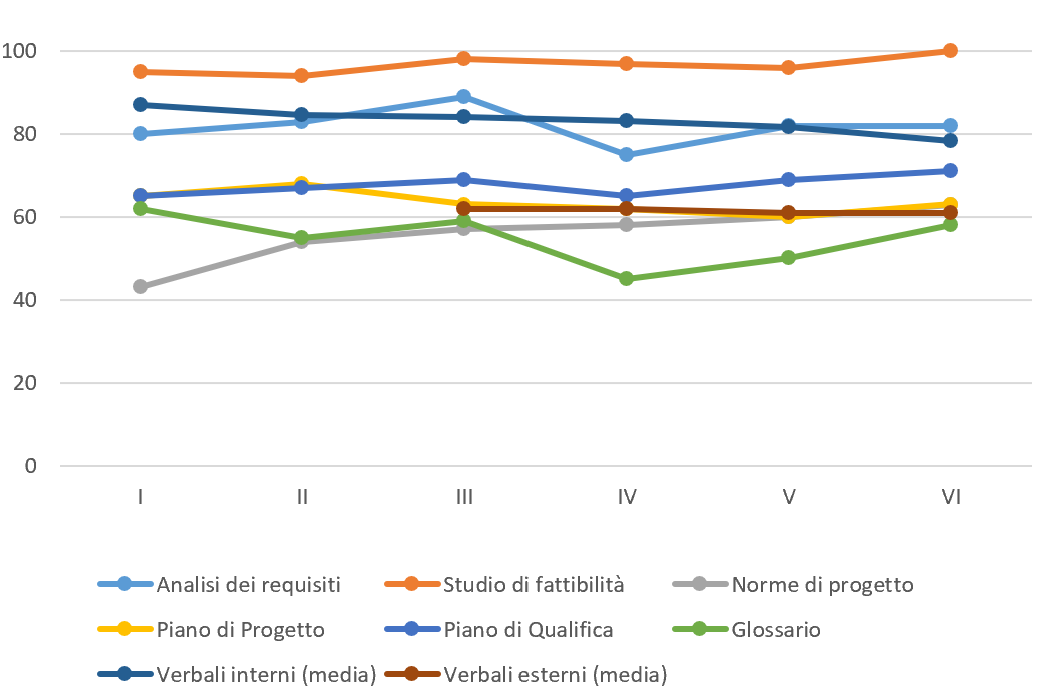
\includegraphics[width=\linewidth]{./img/grafici/2.png}	
	\caption{M-PROD15 revisione dei requisiti}	
\end{figure}
\subsubsection{Esito della revisione esterna}
Il gruppo ritiene poco soddisfacenti i risultati della revisione esterna. 
Le correzioni comunicate attraverso colloqui con i committenti e commenti alla valutazione ci hanno permesso di riflettere sui cambiamenti necessari da mettere in atto sia sui nostri prodotti che sul nostro way of working\glo.
Abbiamo quindi deciso di dare più importanza ai ruoli di verificatore e progettista per non ripetere gli errori della precedente revisione e per sopperire alle carenze segnalate.
Questo non si rifletterà con un aumento delle ore nei ruoli individuati, ma con un maggiore impegno da parte dei componenti del gruppo perché migliori la qualità delle ore svolte e non il numero.

\subsection{Revisione di progettazione (RP)}
\subsubsection{Riassunto delle attività di verifica}
In questo periodo abbiamo attuato le verifiche sui documenti, come nel precedente periodo. A queste abbiamo aggiunto le prime verifiche sulla codifica e sulla pianificazione per verificare che lo svolgimento del progetto\glosp procedesse senza impedimenti.  
\paragraph{Analisi statica dei documenti}
L'analisi statica\glosp dei documenti ha portato alla produzione di una lista degli errori comuni ridotti rispetto alla revisione precedente. Questa lista deve essere aggiornata con le prossime analisi e andrà a facilitare il compito dei verificatori.
\subsubsection{Esiti delle verifiche}
\paragraph{Qualità di processo}
\paragraph*{PRC-Q1 Processo di sviluppo}
\subparagraph{M-PROC01 Scostamento dei requisiti individuati} \mbox{}
\begin{longtable}[H!] {						
		>{}p{50mm}  		
		>{}p{8mm}
		>{}p{8mm}		
		>{}p{8mm}		
		>{}p{8mm}		
		>{}p{8mm}		
		>{}p{8mm}
		>{}p{8mm}
		>{}p{8mm}
		>{}p{8mm}
	}
\rowcolor{gray!50}
\textbf{} & \textbf{I} & \textbf{II} & \textbf{III} & \textbf{IV} & \textbf{V} \TBstrut \\ [2mm]
\textbf{Scostamenti} & 10 & 23 & 29 & 29 & 29 \TBstrut \\ [2mm]
	\rowcolor{white}
\caption{M-PROC01 revisione di progettazione\glo}
\end{longtable}
\begin{figure}[H] 	
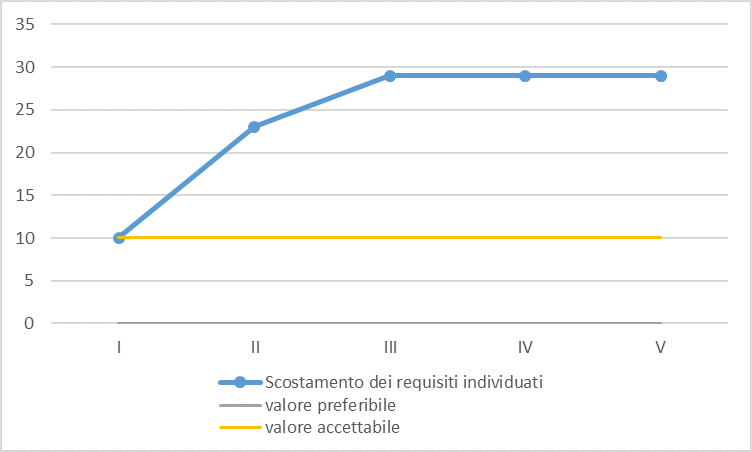
\includegraphics[width=\linewidth]{./img/grafici/RP1.png}	
\caption{M-PROC01 revisione di progettazione\glo}	
\end{figure}
\begin{itemize}
	\item \textbf{Valore preferibile}: 0;
	\item \textbf{Valore accettabile}: 10;
	\item \textbf{Considerazioni}: la metrica\glosp non risulta soddisfatta al termine del periodo di progettazione\glo.
\end{itemize}
\subparagraph{M-PROC02 Numero di parametri per metodo} \mbox{}
\begin{longtable}[H!] {						
		>{}p{50mm}  		
		>{}p{8mm}
		>{}p{8mm}		
		>{}p{8mm}		
		>{}p{8mm}		
		>{}p{8mm}		
		>{}p{8mm}
		>{}p{8mm}
		>{}p{8mm}
		>{}p{8mm}
	}
	\rowcolor{gray!50}
	\textbf{} & \textbf{I} & \textbf{II} & \textbf{III} & \textbf{IV} & \textbf{V} \TBstrut \\ [2mm]
	\textbf{Numero di parametri} & - & - & 3 & 3 & 4 \TBstrut \\ [2mm]
	\rowcolor{white}
	\caption{M-PROC02 revisione di progettazione\glo}
\end{longtable}
\begin{figure}[H] 	
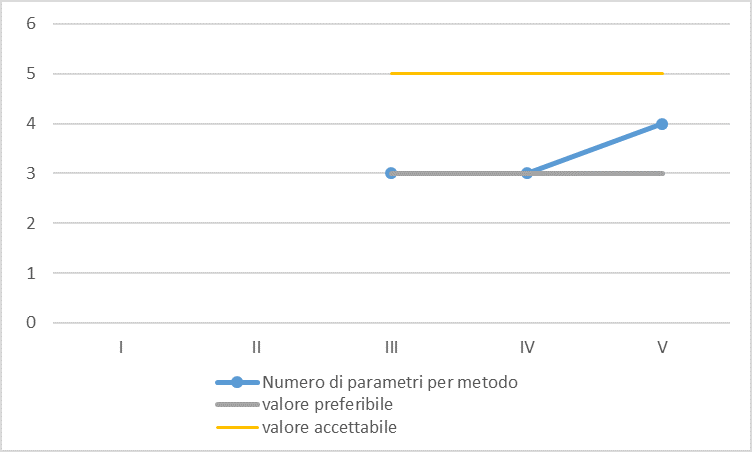
\includegraphics[width=\linewidth]{./img/grafici/RP2.png}	
\caption{M-PROC02 revisione di progettazione\glo}	
\end{figure}
\begin{itemize}
	\item \textbf{Valore preferibile}: $\le3$;
	\item \textbf{Valore accettabile}: $\le5$;
	\item \textbf{Considerazioni}: la metrica\glosp risulta soddisfatta al termine del periodo di progettazione\glo.
\end{itemize}
\pagebreak
\subparagraph{M-PROC03 Numero di metodi per classe} \mbox{}
\begin{longtable}[H!] {						
		>{}p{50mm}  		
		>{}p{8mm}
		>{}p{8mm}		
		>{}p{8mm}		
		>{}p{8mm}		
		>{}p{8mm}		
		>{}p{8mm}
		>{}p{8mm}
		>{}p{8mm}
		>{}p{8mm}
	}
	\rowcolor{gray!50}
	\textbf{} & \textbf{I} & \textbf{II} & \textbf{III} & \textbf{IV} & \textbf{V} \TBstrut \\ [2mm]
	\textbf{Numero di metodi} & - & - & 9 & 9 & 21 \TBstrut \\ [2mm]
	\rowcolor{white}
	\caption{M-PROC03 revisione di progettazione\glo}
\end{longtable}
\begin{figure}[H] 	
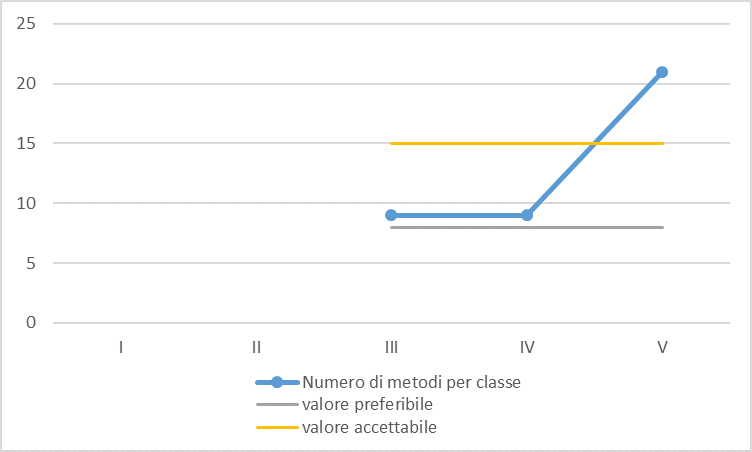
\includegraphics[width=\linewidth]{./img/grafici/RP3.png}	
\caption{M-PROC03 revisione di progettazione\glo}	
\end{figure}
\begin{itemize}
	\item \textbf{Valore preferibile}: $\le8$;
	\item \textbf{Valore accettabile}: $\le15$;
	\item \textbf{Considerazioni}: la metrica\glosp non risulta soddisfatta al termine del periodo di progettazione\glo.
\end{itemize}

\paragraph*{PRC-Q2 Processo di garanzia della qualità}
\subparagraph{M-PROC04 Percentuale di metriche soddisfatte} \mbox{}
\begin{longtable}[H!] {						
		>{}p{50mm}  		
		>{}p{8mm}
		>{}p{8mm}		
		>{}p{8mm}		
		>{}p{8mm}		
		>{}p{8mm}		
		>{}p{8mm}
		>{}p{8mm}
		>{}p{8mm}
		>{}p{8mm}
	}
	\rowcolor{gray!50}
	\textbf{} & \textbf{I} & \textbf{II} & \textbf{III} & \textbf{IV} & \textbf{V} \TBstrut \\ [2mm]
	\textbf{Percentuale} & 58\% & 33\% & 56\% & 72\% & 78\% \TBstrut \\ [2mm]
	\rowcolor{white}
	\caption{M-PROC04 revisione di progettazione\glo}
\end{longtable}
\begin{figure}[H] 	
	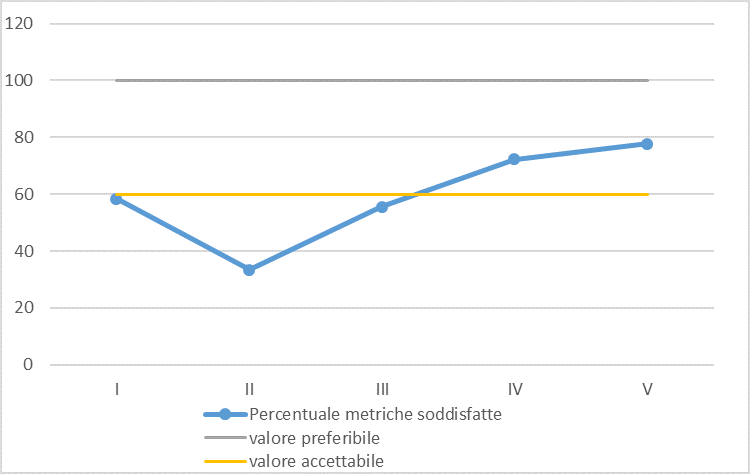
\includegraphics[width=\linewidth]{./img/grafici/RP19.png}	
	\caption{M-PROC04 revisione di progettazione\glo}	
\end{figure}
\begin{itemize}
	\item \textbf{Valore preferibile}: $=100\%$;
	\item \textbf{Valore accettabile}: $\ge60\%$;
	\item \textbf{Considerazioni}: la metrica\glosp risulta soddisfatta al termine del periodo di progettazione\glo.
\end{itemize}
\subparagraph{Considerazioni}
Il gruppo si ritiene soddisfatto rispetto al resoconto della verifica del periodo di progettazione architetturale visto il soddisfacimento della metrica M04. \\
Le metriche\glosp che non sono state soddisfatte al termine del V periodo sono le seguenti:
\begin{itemize}
	\item \textbf{M-PROC01 Scostamento dei requisiti individuati}: viene registrato uno spostamento significativo dei requisiti individuati, il gruppo ha lavorato per una comprendere in modo più approfondito le richieste del proponente per evitare che questo problema possa ripresentarsi in futuro;
	\item \textbf{M-PROC03 Numero di metodi per classe}: il prodotto\glosp dell'attività di codifica per l'implementazione del Proof of Concept\glosp non ha soddisfatto la soglia di accettabilità di questa metrica\glo. Perciò per il prossimo periodo analizzeremo le motivazioni di tale insuccesso per evitare che in futuro si ripresenti questo caso;
	\item \textbf{M-PROD16 Percentuale requisiti obbligatori soddisfatti}: il nostro prodotto\glo, come quindi anche il Proof of Concept\glo, viene realizzato in modo incrementale, perciò in questo periodo questa metrica\glosp non è ancora soddisfatta. Nei prossimi periodi abbiamo pianificato di lavorare con gli incrementi necessari a soddisfare i requisiti obbligatori mancanti;
	\item \textbf{M-PROC05 Percentuale bug sistemati}: il prodotto\glosp dell'attività di codifica per l'implementazione del Proof of Concept\glosp non ha rispettato questa metrica di qualità. Il gruppo ha deciso di analizzare assieme qual'è stato il problema per poterlo risolvere ed evitare che possa verificarsi nuovamente nei prossimi periodi.
\end{itemize}  

\paragraph*{PRC-Q3 Processo di verifica}
\subparagraph{M-PROC05 Percentuale bug sistemati} \mbox{}
\begin{longtable}[H!] {						
		>{}p{50mm}  		
		>{}p{8mm}
		>{}p{8mm}		
		>{}p{8mm}		
		>{}p{8mm}		
		>{}p{8mm}		
		>{}p{8mm}
		>{}p{8mm}
		>{}p{8mm}
		>{}p{8mm}
	}
	\rowcolor{gray!50}
	\textbf{} & \textbf{I} & \textbf{II} & \textbf{III} & \textbf{IV} & \textbf{V} \TBstrut \\ [2mm]
	\textbf{Bug sistemati} & - & - & 0\% & 30\% & 40\% \TBstrut \\ [2mm]
	\rowcolor{white}
	\caption{M-PROC05 revisione di progettazione\glo}
\end{longtable}
\begin{figure}[H] 	
	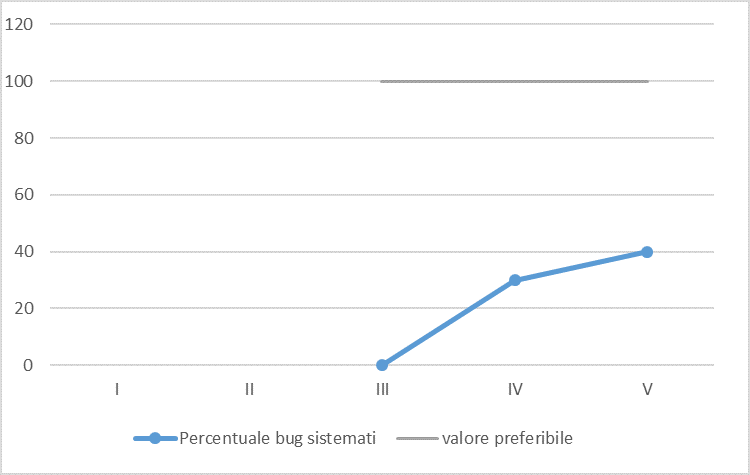
\includegraphics[width=\linewidth]{./img/grafici/RP16.png}	
	\caption{M-PROC05 revisione di progettazione\glo}	
\end{figure}
\begin{itemize}
	\item \textbf{Valore preferibile}: $=100\%$;
	\item \textbf{Valore accettabile}: $=100\%$;
	\item \textbf{Considerazioni}: la metrica\glosp risulta non soddisfatta al termine del periodo di progettazione\glo.
\end{itemize}

\paragraph*{PRC-Q4 Processo di gestione dei cambiamenti}
\subparagraph{M-PROC06 Tempo medio risoluzione errori} \mbox{}
\begin{longtable}[H!] {						
		>{}p{38mm}  		
		>{}p{12mm}
		>{}p{12mm}		
		>{}p{12mm}		
		>{}p{12mm}		
		>{}p{12mm}		
		>{}p{12mm}
		>{}p{12mm}
		>{}p{12mm}
		>{}p{12mm}
	}
	\rowcolor{gray!50}
	\textbf{} & \textbf{I} & \textbf{II} & \textbf{III} & \textbf{IV} & \textbf{V} \TBstrut \\ [2mm]
	\textbf{Tempo medio} & 15min & 134min & 122min & 110min & 104min \TBstrut \\ [2mm]
	\rowcolor{white}
	\caption{M-PROC06 revisione di progettazione\glo}
\end{longtable}
\begin{figure}[H] 	
	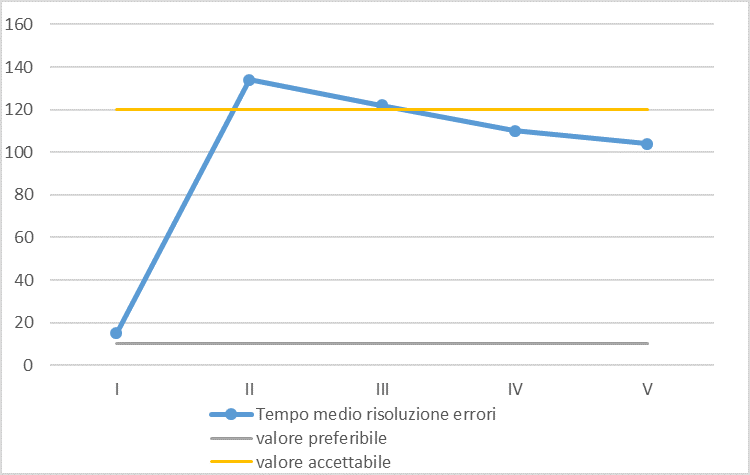
\includegraphics[width=\linewidth]{./img/grafici/RP12.png}	
	\caption{M-PROC06 revisione di progettazione\glo}	
\end{figure}
\begin{itemize}
	\item \textbf{Valore preferibile}: $\le10minuti$;
	\item \textbf{Valore accettabile}: $\le120minuti$;
	\item \textbf{Considerazioni}: la metrica\glosp risulta soddisfatta al termine del periodo di progettazione\glo.
\end{itemize}

\paragraph*{PRC-Q5 Processo di gestione organizzativa}
\subparagraph{M-PROC07 Planned value} \mbox{}
\begin{longtable}[H!] {						
		>{}p{38mm}  		
		>{}p{12mm}
		>{}p{12mm}		
		>{}p{12mm}		
		>{}p{12mm}		
		>{}p{12mm}		
		>{}p{12mm}
		>{}p{12mm}
		>{}p{12mm}
		>{}p{12mm}
	}
	\rowcolor{gray!50}
	\textbf{} & \textbf{I} & \textbf{II} & \textbf{III} & \textbf{IV} & \textbf{V} \TBstrut \\ [2mm]
	\textbf{PV} & 800\euro & 1868\euro & 2401\euro & 3068\euro & 3836\euro \TBstrut \\ [2mm]
	\rowcolor{white}
	\caption{M-PROC07 revisione di progettazione\glo}
\end{longtable}
\begin{figure}[H] 	
	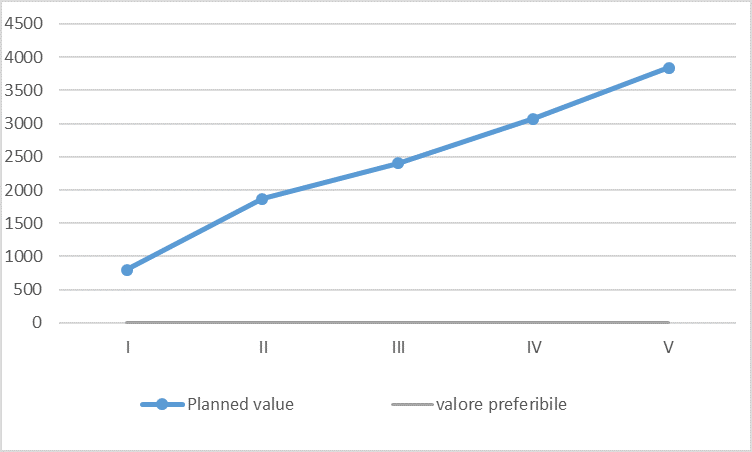
\includegraphics[width=\linewidth]{./img/grafici/RP4.png}	
	\caption{M-PROC07 revisione di progettazione\glo}	
\end{figure}
\begin{itemize}
	\item \textbf{Valore preferibile}: $\ge0$;
	\item \textbf{Valore accettabile}: $\ge0$;
	\item \textbf{Considerazioni}: la metrica\glosp risulta soddisfatta al termine del periodo di progettazione\glo.
\end{itemize}
\subparagraph{M-PROC08 Earned value} \mbox{}
\begin{longtable}[H!] {						
		>{}p{38mm}  		
		>{}p{12mm}
		>{}p{12mm}		
		>{}p{12mm}		
		>{}p{12mm}		
		>{}p{12mm}		
		>{}p{12mm}
		>{}p{12mm}
		>{}p{12mm}
		>{}p{12mm}
	}
	\rowcolor{gray!50}
	\textbf{} & \textbf{I} & \textbf{II} & \textbf{III} & \textbf{IV} & \textbf{V} \TBstrut \\ [2mm]
	\textbf{EV} & 650\euro & 1300\euro & 2380\euro & 3050\euro & 3836\euro \TBstrut \\ [2mm]
	\rowcolor{white}
	\caption{M-PROC08 revisione di progettazione\glo}
\end{longtable}
\begin{figure}[H] 	
	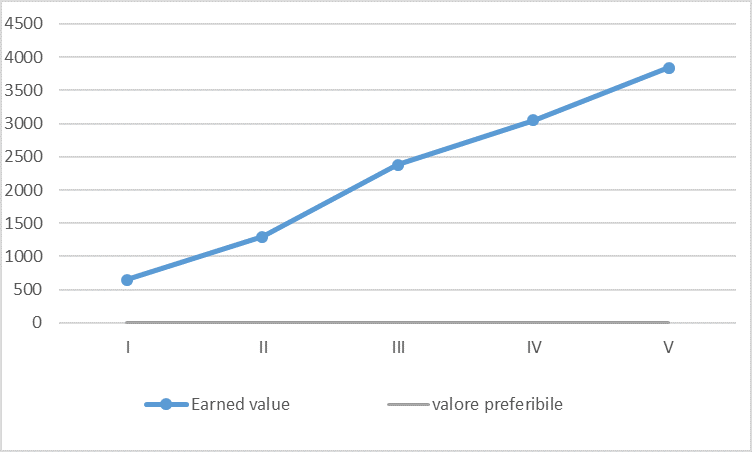
\includegraphics[width=\linewidth]{./img/grafici/RP5.png}	
	\caption{M-PROC08 revisione di progettazione\glo}	
\end{figure}
\begin{itemize}
	\item \textbf{Valore preferibile}: $\ge0$;
	\item \textbf{Valore accettabile}: $\ge0$;
	\item \textbf{Considerazioni}: la metrica\glosp risulta soddisfatta al termine del periodo di progettazione\glo.
\end{itemize}
\subparagraph{M-PROC09 Actual cost} \mbox{}
\begin{longtable}[H!] {						
		>{}p{38mm}  		
		>{}p{12mm}
		>{}p{12mm}		
		>{}p{12mm}		
		>{}p{12mm}		
		>{}p{12mm}		
		>{}p{12mm}
		>{}p{12mm}
		>{}p{12mm}
		>{}p{12mm}
	}
	\rowcolor{gray!50}
	\textbf{} & \textbf{I} & \textbf{II} & \textbf{III} & \textbf{IV} & \textbf{V} \TBstrut \\ [2mm]
	\textbf{AC} & 1021\euro & 1982\euro & 2582\euro & 3086\euro & 3836\euro \TBstrut \\ [2mm]
	\rowcolor{white}
	\caption{M-PROC09 revisione di progettazione\glo}
\end{longtable}
\begin{figure}[H] 	
	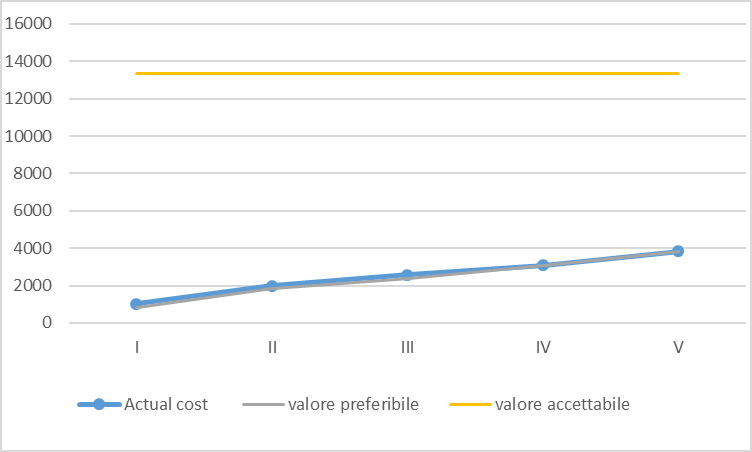
\includegraphics[width=\linewidth]{./img/grafici/RP6.png}	
	\caption{M-PROC09 revisione di progettazione\glo}	
	\begin{itemize}
		\item \textbf{Valore preferibile}: $0\le AC \le PV$;
		\item \textbf{Valore accettabile}: $0 \le AC \le budget \; totale$;
		\item \textbf{Considerazioni}: la metrica\glosp risulta soddisfatta al termine del periodo di progettazione\glo.
	\end{itemize}
\end{figure}
\subparagraph{M-PROC10 Cost performance index} \mbox{}
\begin{longtable}[H!] {						
		>{}p{50mm}  		
		>{}p{8mm}
		>{}p{8mm}		
		>{}p{8mm}		
		>{}p{8mm}		
		>{}p{8mm}		
		>{}p{8mm}
		>{}p{8mm}
		>{}p{8mm}
		>{}p{8mm}
	}
	\rowcolor{gray!50}
	\textbf{} & \textbf{I} & \textbf{II} & \textbf{III} & \textbf{IV} & \textbf{V} \TBstrut \\ [2mm]
	\textbf{CPI} & 0,64 & 0,66 & 0,92 & 0,99 & 1 \TBstrut \\ [2mm]
	\rowcolor{white}
	\caption{M-PROC10 revisione di progettazione\glo}
\end{longtable}
\begin{figure}[H] 	
	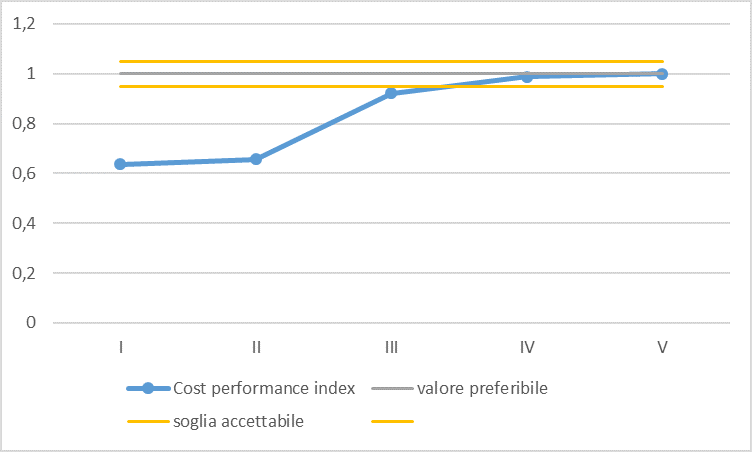
\includegraphics[width=\linewidth]{./img/grafici/RP7.png}	
	\caption{M-PROC10 revisione di progettazione\glo}	
\end{figure}
\begin{itemize}
	\item \textbf{Valore preferibile}: $=1$;
	\item \textbf{Valore accettabile}: $0.95 \le CPI \le 1.05$;
	\item \textbf{Considerazioni}: la metrica\glosp risulta soddisfatta al termine del periodo di progettazione\glo.
\end{itemize}
\subparagraph{M-PROC11 Schedule performance index} \mbox{}
\begin{longtable}[H!] {						
		>{}p{50mm}  		
		>{}p{8mm}
		>{}p{8mm}		
		>{}p{8mm}		
		>{}p{8mm}		
		>{}p{8mm}		
		>{}p{8mm}
		>{}p{8mm}
		>{}p{8mm}
		>{}p{8mm}
	}
	\rowcolor{gray!50}
	\textbf{} & \textbf{I} & \textbf{II} & \textbf{III} & \textbf{IV} & \textbf{V} \TBstrut \\ [2mm]
	\textbf{SPI} & 0,81 & 0,69 & 0,99 & 0,99 & 1 \TBstrut \\ [2mm]
	\rowcolor{white}
	\caption{M-PROC11 revisione di progettazione\glo}
\end{longtable}
\begin{figure}[H] 	
	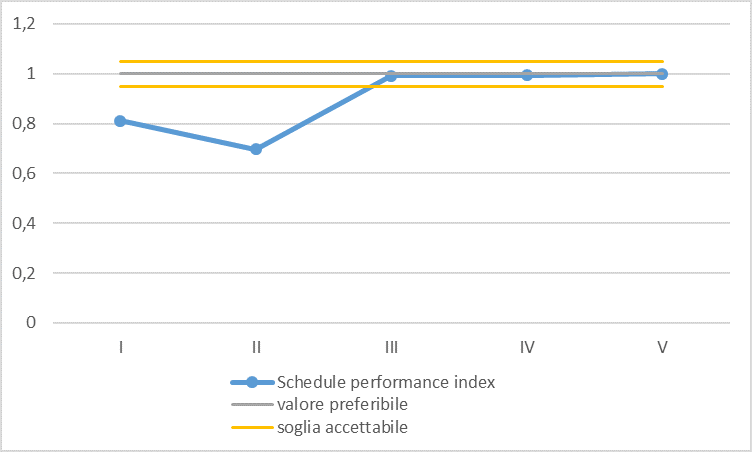
\includegraphics[width=\linewidth]{./img/grafici/RP8.png}	
	\caption{M-PROC11 revisione di progettazione\glo}	
\end{figure}
\begin{itemize}
	\item \textbf{Valore preferibile}: $=1$;
	\item \textbf{Valore accettabile}: $0.95 \le SPI \le 1.05$;
	\item \textbf{Considerazioni}: la metrica\glosp risulta soddisfatta al termine del periodo di progettazione\glo.
\end{itemize}
\subparagraph{M-PROC12 Estimated cost at compltion} \mbox{}
\begin{longtable}[H!] {						
		>{}p{38mm}  		
		>{}p{12mm}
		>{}p{12mm}		
		>{}p{12mm}		
		>{}p{12mm}		
		>{}p{12mm}		
		>{}p{12mm}
		>{}p{12mm}
		>{}p{12mm}
		>{}p{12mm}
	}
	\rowcolor{gray!50}
	\textbf{} & \textbf{I} & \textbf{II} & \textbf{III} & \textbf{IV} & \textbf{V} \TBstrut \\ [2mm]
	\textbf{EAC} & 20955\euro & 20340\euro & 14473\euro & 13498\euro & 13341\euro \TBstrut \\ [2mm]
	\rowcolor{white}
	\caption{M-PROC12 revisione di progettazione\glo}
\end{longtable}
\begin{figure}[H] 	
	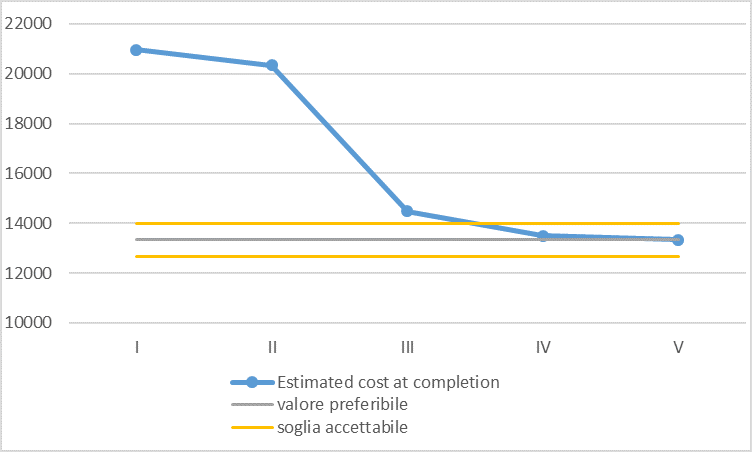
\includegraphics[width=\linewidth]{./img/grafici/RP9.png}	
	\caption{M-PROC12 revisione di progettazione\glo}	
\end{figure}
\begin{itemize}
	\item \textbf{Valore preferibile}: pari a quanto preventivato;
	\item \textbf{Valore accettabile}: $preventivo-5\% \le EAC \le preventivo+5\%$;
	\item \textbf{Considerazioni}: la metrica\glosp risulta soddisfatta al termine del periodo di progettazione\glo.
\end{itemize}
\subparagraph{M-PROC13 Schedule at completion} \mbox{}
\begin{longtable}[H!] {						
		>{}p{18mm}  		
		>{}p{16mm}
		>{}p{16mm}		
		>{}p{16mm}		
		>{}p{16mm}		
		>{}p{16mm}		
		>{}p{16mm}
		>{}p{16mm}
		>{}p{16mm}
		>{}p{16mm}
	}
	\rowcolor{gray!50}
	\textbf{} & \textbf{I} & \textbf{II} & \textbf{III} & \textbf{IV} & \textbf{V} \TBstrut \\ [2mm]
	\textbf{SAC} & 879 ore & 1026 ore & 720 ore & 718 ore & 714 ore \TBstrut \\ [2mm]
	\rowcolor{white}
	\caption{M-PROC13 revisione di progettazione\glo}
\end{longtable}
\begin{figure}[H] 	
	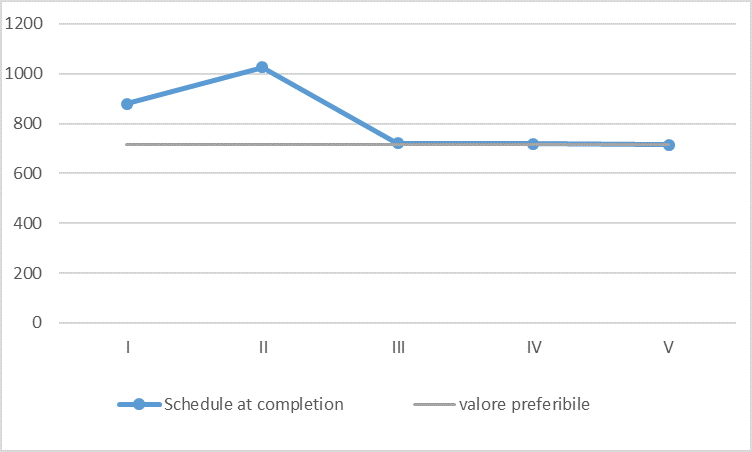
\includegraphics[width=\linewidth]{./img/grafici/RP10.png}	
	\caption{M-PROC13 revisione di progettazione\glo}	
\end{figure}
\begin{itemize}
	\item \textbf{Valore preferibile}: pari a quanto preventivato;
	\item \textbf{Valore accettabile}: pari a quanto preventivato;
	\item \textbf{Considerazioni}: la metrica\glosp risulta soddisfatta al termine del periodo di progettazione\glo.
\end{itemize}
\subparagraph{M-PROC14 Rischi non preventivati} \mbox{}
\begin{longtable}[H!] {						
		>{}p{50mm}  		
		>{}p{8mm}
		>{}p{8mm}		
		>{}p{8mm}		
		>{}p{8mm}		
		>{}p{8mm}		
		>{}p{8mm}
		>{}p{8mm}
		>{}p{8mm}
		>{}p{8mm}
	}
	\rowcolor{gray!50}
	\textbf{} & \textbf{I} & \textbf{II} & \textbf{III} & \textbf{IV} & \textbf{V} \TBstrut \\ [2mm]
	\textbf{Rischi} & 0 & 0 & 0 & 0 & 0 \TBstrut \\ [2mm]
	\rowcolor{white}
	\caption{M-PROC14 revisione di progettazione\glo}
\end{longtable}
\begin{figure}[H] 	
	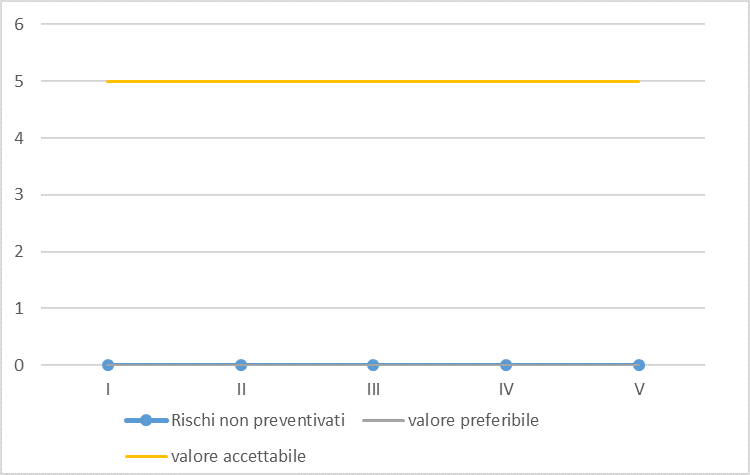
\includegraphics[width=\linewidth]{./img/grafici/RP11.png}	
	\caption{M-PROC14 revisione di progettazione\glo}	
\end{figure}
\begin{itemize}
	\item \textbf{Valore preferibile}: $=0$;
	\item \textbf{Valore accettabile}: $\le 5$;
	\item \textbf{Considerazioni}: la metrica\glosp risulta soddisfatta al termine del periodo di progettazione\glo.
\end{itemize}

\paragraph{Qualità di prodotto}
\paragraph*{PRD-Q1 Documenti}
\subparagraph{M-PROD15 Indice di Gulpease}\mbox{}
\begin{longtable} {						
		>{}p{50mm}  		
		>{}p{8mm}		
		>{}p{8mm}		
		>{}p{8mm}		
		>{}p{8mm}		
		>{}p{8mm}		
		>{}p{8mm}
		>{}p{8mm}
		>{}p{8mm}
		>{}p{8mm}				
	}			
	\rowcolor{gray!50}
	\textbf{Documento} & \textbf{I} & \textbf{II} & \textbf{III} & \textbf{IV} & \textbf{V} \TBstrut \\ [2mm]
	\textbf{Analisi dei Requisiti} & 93 & 100 & 100 & 100 & 100 \TBstrut \\ [2mm]
	\textbf{Norme di Progetto} & 73 & 79 & 79 & 79 & 81 \TBstrut \\ [2mm]
	\textbf{Piano di Progetto} & 82 & 92 & 75 & 94 & 97 \TBstrut \\ [2mm]
	\textbf{Piano di Qualifica} & 89 & 91 & 87 & 92 & 95 \TBstrut \\ [2mm]
	\textbf{Glossario} & 58 & 83 & 83 & 83 & 83 \TBstrut \\ [2mm]
	\textbf{Verbali interni (media)} & - & 100 & 100 & 100 & 100 \TBstrut \\ [2mm]
	\textbf{Verbali esterni (media)} & - & - & 97 & 97 & 98 \TBstrut \\ [2mm]
	\rowcolor{white}
	\caption{M-PROD15 revisione di progettazione\glo}
\end{longtable}
\begin{figure}[H] 	
	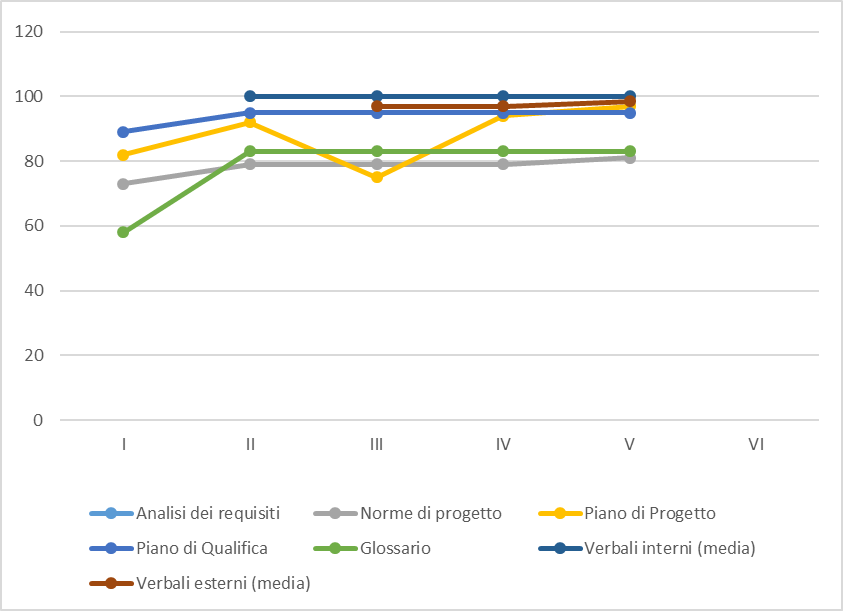
\includegraphics[width=\linewidth]{./img/grafici/RP18.png}	
	\caption{M-PROD15 revisione di progettazione\glo}	
\end{figure}
\begin{longtable} {						
		>{}p{70mm}  		
		>{}p{8mm}		
		>{}p{8mm}		
		>{}p{8mm}		
		>{}p{8mm}		
		>{}p{8mm}		
		>{}p{8mm}
		>{}p{8mm}
		>{}p{8mm}
		>{}p{8mm}				
	}			
	\rowcolor{gray!50}
	\textbf{} & \textbf{I} & \textbf{II} & \textbf{III} & \textbf{IV} & \textbf{V} \TBstrut \\ [2mm]
	\textbf{Media dell'indice di Gulpease} & 79 & 90 & 89 & 92 & 93 \TBstrut \\ [2mm]
	\rowcolor{white}
	\caption{M-PROD15 revisione di progettazione\glo}
\end{longtable}
\begin{figure}[H] 	
	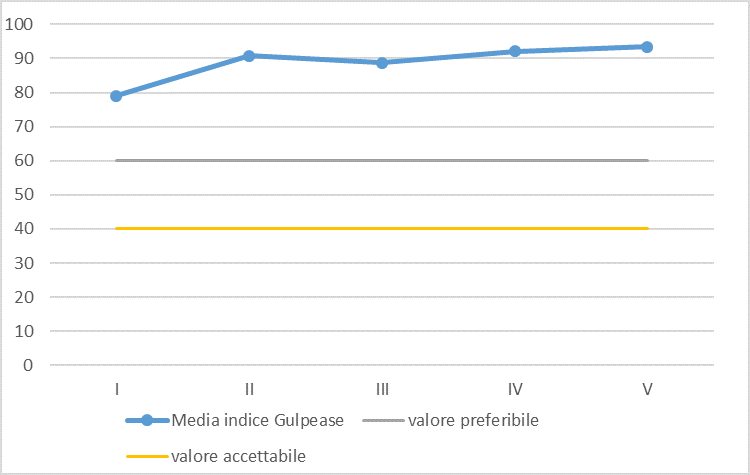
\includegraphics[width=\linewidth]{./img/grafici/RP20.png}	
	\caption{M-PROD15 revisione di progettazione\glo}	
\end{figure}
\begin{itemize}
	\item \textbf{Valore preferibile}: $\ge60$;
	\item \textbf{Valore accettabile}: $\ge40$;
	\item \textbf{Considerazioni}: la metrica\glosp risulta soddisfatta al termine del periodo di progettazione\glo.
\end{itemize}
\subparagraph{M-PROD19 Correttezza ortografica} \mbox{}
\begin{longtable}[H!] {						
		>{}p{50mm}  		
		>{}p{8mm}
		>{}p{8mm}		
		>{}p{8mm}		
		>{}p{8mm}		
		>{}p{8mm}		
		>{}p{8mm}
		>{}p{8mm}
		>{}p{8mm}
		>{}p{8mm}
	}
	\rowcolor{gray!50}
	\textbf{} & \textbf{I} & \textbf{II} & \textbf{III} & \textbf{IV} & \textbf{V} \TBstrut \\ [2mm]
	\textbf{Numero di metodi} & 0 & 1 & 0 & 0 & 0 \TBstrut \\ [2mm]
	\rowcolor{white}
	\caption{M-PROD19 revisione di progettazione\glo}
\end{longtable}
\begin{figure}[H] 	
	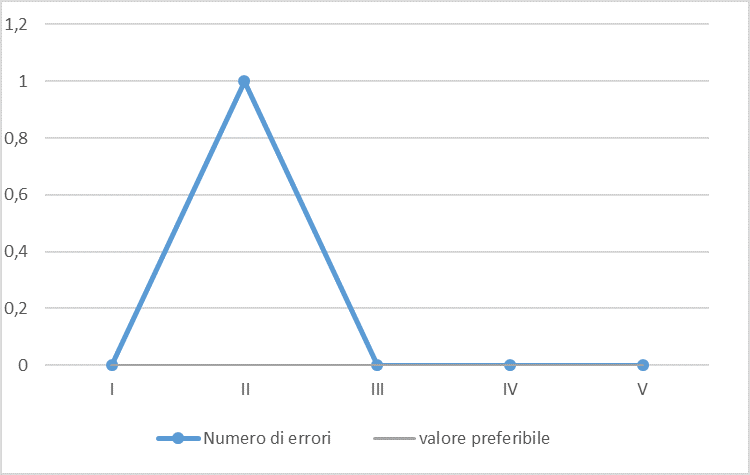
\includegraphics[width=\linewidth]{./img/grafici/RP17.png}	
	\caption{M-PROD19 revisione di progettazione\glo}	
\end{figure}
\begin{itemize}
	\item \textbf{Valore preferibile}: $=0$;
	\item \textbf{Valore accettabile}: $=0$;
	\item \textbf{Considerazioni}: la metrica\glosp risulta soddisfatta al termine del periodo di progettazione\glo.
\end{itemize}
\paragraph*{PRD-Q2 Appropriatezza funzionale}
\subparagraph{M-PROD16 Percentuale di requisiti obbligatori soddisfatti} \mbox{}
\begin{longtable}[H!] {						
		>{}p{50mm}  		
		>{}p{8mm}
		>{}p{8mm}		
		>{}p{8mm}		
		>{}p{8mm}		
		>{}p{8mm}		
		>{}p{8mm}
		>{}p{8mm}
		>{}p{8mm}
		>{}p{8mm}
	}
	\rowcolor{gray!50}
	\textbf{} & \textbf{I} & \textbf{II} & \textbf{III} & \textbf{IV} & \textbf{V} \TBstrut \\ [2mm]
	\textbf{PROS} & - & - & 32\% & 53\% & 53\% \TBstrut \\ [2mm]
	\rowcolor{white}
	\caption{M-PROD16 revisione di progettazione\glo}
\end{longtable}
\begin{figure}[H] 	
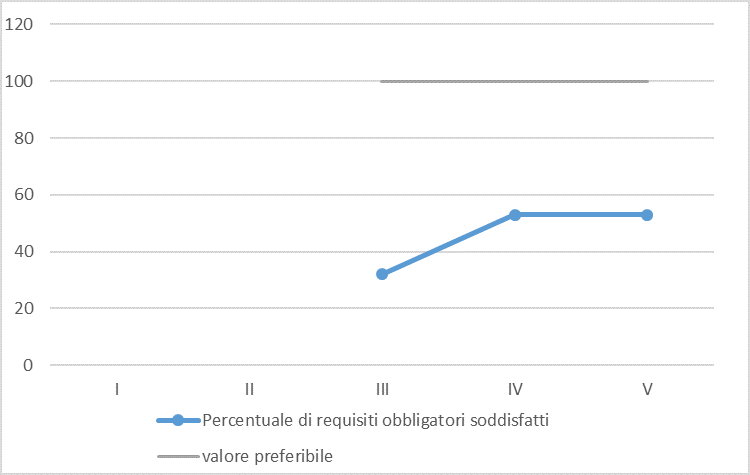
\includegraphics[width=\linewidth]{./img/grafici/RP13.png}	
\caption{M-PROD16 revisione di progettazione\glo}	
\end{figure}
\begin{itemize}
	\item \textbf{Valore preferibile}: $=100\%$;
	\item \textbf{Valore accettabile}: $=100\%$;
	\item \textbf{Considerazioni}: la metrica\glosp risulta non soddisfatta al termine del periodo di progettazione\glo.
\end{itemize}
\subparagraph{M-PROD17 Percentuale di requisiti desiderabili soddisfatti} \mbox{}
\begin{longtable}[H!] {						
		>{}p{50mm}  		
		>{}p{8mm}
		>{}p{8mm}		
		>{}p{8mm}		
		>{}p{8mm}		
		>{}p{8mm}		
		>{}p{8mm}
		>{}p{8mm}
		>{}p{8mm}
		>{}p{8mm}
	}
	\rowcolor{gray!50}
	\textbf{} & \textbf{I} & \textbf{II} & \textbf{III} & \textbf{IV} & \textbf{V} \TBstrut \\ [2mm]
	\textbf{PRDS} & - & - & 0\% & 0\% & 0\% \TBstrut \\ [2mm]
	\rowcolor{white}
	\caption{M-PROD17 revisione di progettazione\glo}
\end{longtable}
\begin{figure}[H] 	
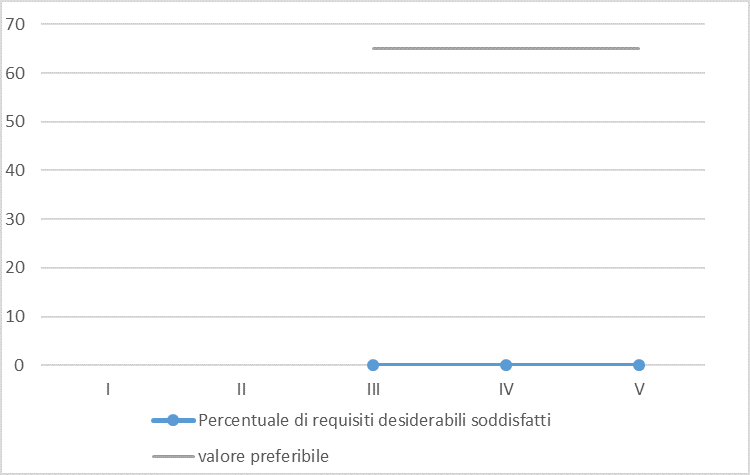
\includegraphics[width=\linewidth]{./img/grafici/RP14.png}	
\caption{M-PROD17 revisione di progettazione\glo}	
\end{figure}
\begin{itemize}
	\item \textbf{Valore preferibile}: $\ge 65\%$;
	\item \textbf{Valore accettabile}: $\ge 0\%$;
	\item \textbf{Considerazioni}: la metrica\glosp risulta soddisfatta al termine del periodo di progettazione\glo.
\end{itemize}
\subparagraph{M-PROD18 Percentuale di requisiti opzionali soddisfatti} \mbox{}
\begin{longtable}[H!] {						
		>{}p{50mm}  		
		>{}p{8mm}
		>{}p{8mm}		
		>{}p{8mm}		
		>{}p{8mm}		
		>{}p{8mm}		
		>{}p{8mm}
		>{}p{8mm}
		>{}p{8mm}
		>{}p{8mm}
	}
	\rowcolor{gray!50}
	\textbf{} & \textbf{I} & \textbf{II} & \textbf{III} & \textbf{IV} & \textbf{V} \TBstrut \\ [2mm]
	\textbf{PROpS} & - & - & 0\% & 0\% & 0\% \TBstrut \\ [2mm]
	\rowcolor{white}
	\caption{M-PROD18 revisione di progettazione\glo}
\end{longtable}
\begin{figure}[H] 	
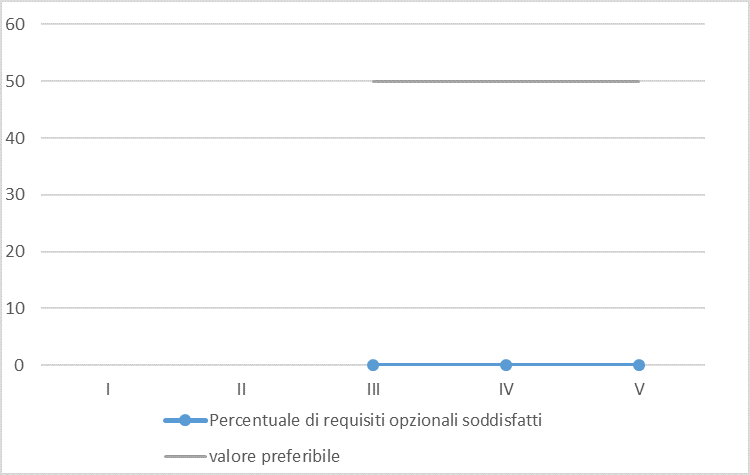
\includegraphics[width=\linewidth]{./img/grafici/RP15.png}	
\caption{M-PROD18 revisione di progettazione\glo}	
\end{figure}
\begin{itemize}
	\item \textbf{Valore preferibile}: $\ge50\%$;
	\item \textbf{Valore accettabile}: $\ge0\%$;
	\item \textbf{Considerazioni}: la metrica\glosp risulta soddisfatta al termine del periodo di progettazione\glo.
\end{itemize}
\subsection{Revisione di qualifica (RQ)}
\subsubsection{Riassunto delle attività di verifica}
In questo periodo abbiamo attuato le verifiche sui documenti, sulla codifica e sulla pianificazione come nel precedente periodo. A queste abbiamo aggiunto le verifiche sulla progettazione e sui testi per verificare che lo svolgimento del progetto\glosp procedesse senza impedimenti.  
\paragraph{Analisi statica dei documenti}
L'analisi statica\glosp dei documenti ha portato alla produzione di una lista degli errori comuni ridotti rispetto alla revisione precedente. Questa lista deve essere aggiornata con le prossime analisi e andrà a facilitare il compito dei verificatori.
\subsubsection{Esiti delle verifiche} 
\paragraph{Qualità di processo}
\paragraph*{PRC-Q1 Processo di sviluppo}
\subparagraph{M-PROC01 Scostamento dei requisiti individuati} \mbox{}
\begin{longtable}[H!] {						
		>{}p{50mm}  		
		>{}p{8mm}
		>{}p{8mm}		
		>{}p{8mm}		
		>{}p{8mm}		
		>{}p{8mm}		
		>{}p{8mm}
		>{}p{8mm}
		>{}p{8mm}
		>{}p{8mm}
	}
	\rowcolor{gray!50}
	\textbf{} & \textbf{I} & \textbf{II} & \textbf{III} & \textbf{IV} & \textbf{V} & \textbf{VI} \TBstrut \\ [2mm]
	\textbf{Scostamenti} & 1 & 0 & 0 & 0 & 0 & 0 \TBstrut \\ [2mm]
	\rowcolor{white}
	\caption{M-PROC01 revisione di qualifica}
\end{longtable}
\begin{figure}[H] 	
	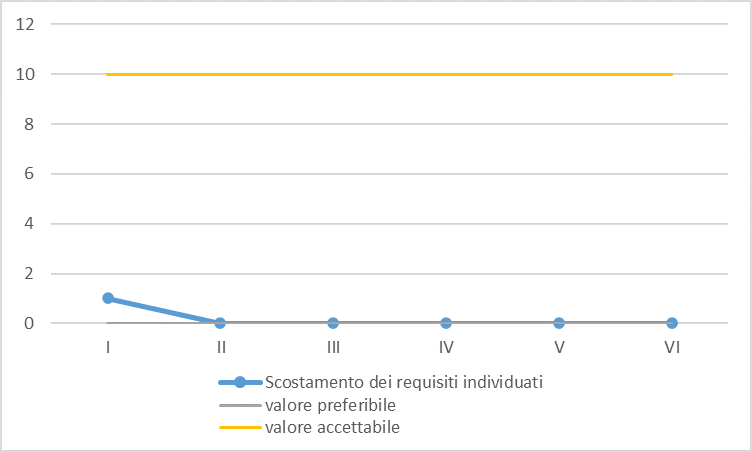
\includegraphics[width=\linewidth]{./img/grafici/RQ1.png}	
	\caption{M-PROC01 revisione di qualifica}	
\end{figure}
\begin{itemize}
	\item \textbf{Valore preferibile}: 0;
	\item \textbf{Valore accettabile}: 10;
	\item \textbf{Considerazioni}: la metrica\glosp risulta soddisfatta al termine del periodo di qualifica.
\end{itemize}

\subparagraph{M-PROC02 Numero di parametri per metodo} \mbox{}
\begin{longtable}[H!] {						
		>{}p{50mm}  		
		>{}p{8mm}
		>{}p{8mm}		
		>{}p{8mm}		
		>{}p{8mm}		
		>{}p{8mm}		
		>{}p{8mm}
		>{}p{8mm}
		>{}p{8mm}
		>{}p{8mm}
	}
	\rowcolor{gray!50}
	\textbf{} & \textbf{I} & \textbf{II} & \textbf{III} & \textbf{IV} & \textbf{V} & \textbf{VI} \TBstrut \\ [2mm]
	\textbf{Numero} & 4 & 5 & 5 & 5 & 5 & 5 \TBstrut \\ [2mm]
	\rowcolor{white}
	\caption{M-PROC02 revisione di qualifica}
\end{longtable}
\begin{figure}[H] 	
	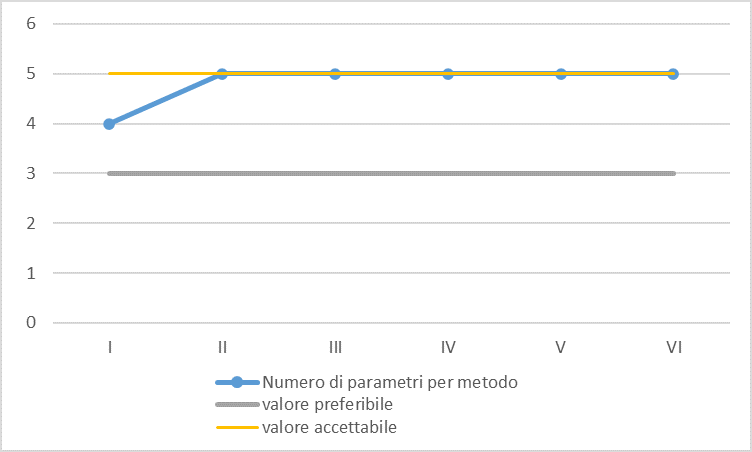
\includegraphics[width=\linewidth]{./img/grafici/RQ2.png}	
	\caption{M-PROC02 revisione di qualifica}	
\end{figure}
\begin{itemize}
	\item \textbf{Valore preferibile}: $\le 3$;
	\item \textbf{Valore accettabile}: $\le 5$;
	\item \textbf{Considerazioni}: la metrica\glosp risulta soddisfatta al termine del periodo di qualifica.
\end{itemize}

\subparagraph{M-PROC03 Numero di metodi per classe} \mbox{}
\begin{longtable}[H!] {						
		>{}p{50mm}  		
		>{}p{8mm}
		>{}p{8mm}		
		>{}p{8mm}		
		>{}p{8mm}		
		>{}p{8mm}		
		>{}p{8mm}
		>{}p{8mm}
		>{}p{8mm}
		>{}p{8mm}
	}
	\rowcolor{gray!50}
	\textbf{} & \textbf{I} & \textbf{II} & \textbf{III} & \textbf{IV} & \textbf{V} & \textbf{VI} \TBstrut \\ [2mm]
	\textbf{Numero} & 15 & 15 & 15 & 14 & 16 & 15 \TBstrut \\ [2mm]
	\rowcolor{white}
	\caption{M-PROC03 revisione di qualifica}
\end{longtable}
\begin{figure}[H] 	
	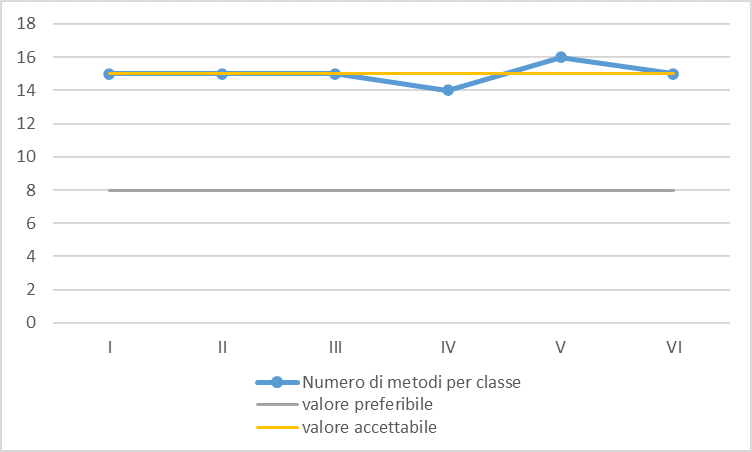
\includegraphics[width=\linewidth]{./img/grafici/RQ3.png}	
	\caption{M-PROC03 revisione di qualifica}	
\end{figure}
\begin{itemize}
	\item \textbf{Valore preferibile}: $\le 8$;
	\item \textbf{Valore accettabile}: $\le 15$;
	\item \textbf{Considerazioni}: la metrica\glosp risulta soddisfatta al termine del periodo di qualifica.
\end{itemize}

\subparagraph{M-PROC20 Livello di annidamento} \mbox{}
\begin{longtable}[H!] {						
		>{}p{50mm}  		
		>{}p{8mm}
		>{}p{8mm}		
		>{}p{8mm}		
		>{}p{8mm}		
		>{}p{8mm}		
		>{}p{8mm}
		>{}p{8mm}
		>{}p{8mm}
		>{}p{8mm}
	}
	\rowcolor{gray!50}
	\textbf{} & \textbf{I} & \textbf{II} & \textbf{III} & \textbf{IV} & \textbf{V} & \textbf{VI} \TBstrut \\ [2mm]
	\textbf{Livello} & 1 & 1 & 2 & 2 & 2 & 2 \TBstrut \\ [2mm]
	\rowcolor{white}
	\caption{M-PROC20 revisione di qualifica}
\end{longtable}
\begin{figure}[H] 	
	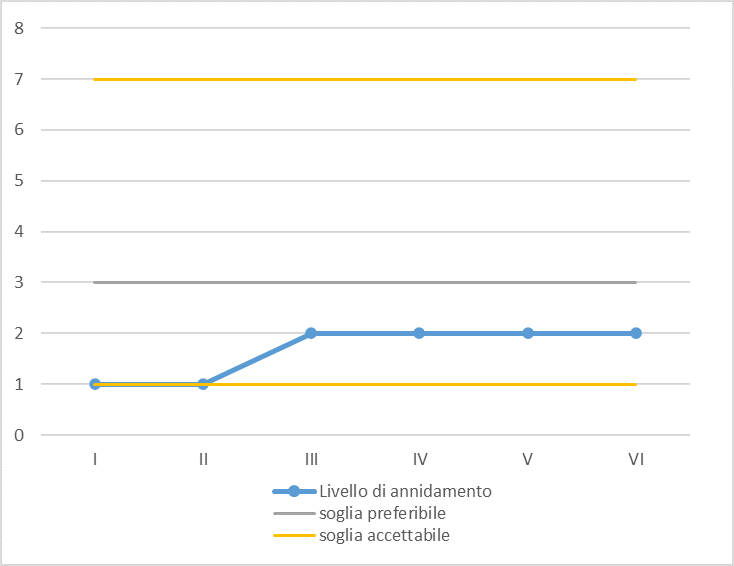
\includegraphics[width=\linewidth]{./img/grafici/RQ20.png}	
	\caption{M-PROC20 revisione di qualifica}	
\end{figure}
\begin{itemize}
	\item \textbf{Valore preferibile}: $1\le x \le 3$;
	\item \textbf{Valore accettabile}: $1 \le x \le 7$;
	\item \textbf{Considerazioni}: la metrica\glosp risulta soddisfatta al termine del periodo di qualifica.
\end{itemize}
\subparagraph{M-PROC21 Profondità gerarchia} \mbox{}
\begin{longtable}[H!] {						
		>{}p{50mm}  		
		>{}p{8mm}
		>{}p{8mm}		
		>{}p{8mm}		
		>{}p{8mm}		
		>{}p{8mm}		
		>{}p{8mm}
		>{}p{8mm}
		>{}p{8mm}
		>{}p{8mm}
	}
	\rowcolor{gray!50}
	\textbf{} & \textbf{I} & \textbf{II} & \textbf{III} & \textbf{IV} & \textbf{V} & \textbf{VI} \TBstrut \\ [2mm]
	\textbf{Profondità} & 2 & 2 & 2 & 2 & 2 & 2 \TBstrut \\ [2mm]
	\rowcolor{white}
	\caption{M-PROC21 revisione di qualifica}
\end{longtable}
\begin{figure}[H] 	
	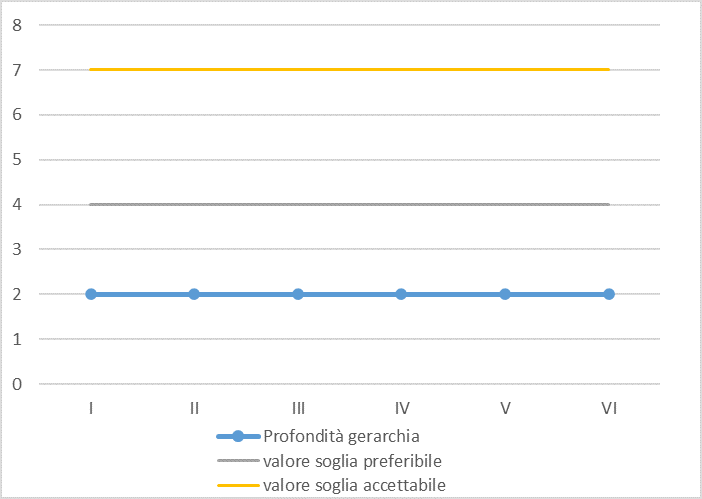
\includegraphics[width=\linewidth]{./img/grafici/RQ21.png}	
	\caption{M-PROC21 revisione di qualifica}	
\end{figure}
\begin{itemize}
	\item \textbf{Valore preferibile}: $\le 4$;
	\item \textbf{Valore accettabile}: $\le 7$;
	\item \textbf{Considerazioni}: la metrica\glosp risulta soddisfatta al termine del periodo di qualifica.
\end{itemize}

\subparagraph{M-PROC22 Numero di design pattern} \mbox{}
\begin{longtable}[H!] {						
		>{}p{50mm}  		
		>{}p{8mm}
		>{}p{8mm}		
		>{}p{8mm}		
		>{}p{8mm}		
		>{}p{8mm}		
		>{}p{8mm}
		>{}p{8mm}
		>{}p{8mm}
		>{}p{8mm}
	}
	\rowcolor{gray!50}
	\textbf{} & \textbf{I} & \textbf{II} & \textbf{III} & \textbf{IV} & \textbf{V} & \textbf{VI} \TBstrut \\ [2mm]
	\textbf{Numero} & 4 & 6 & 6 & 6 & 6 & 6 \TBstrut \\ [2mm]
	\rowcolor{white}
	\caption{M-PROC22 revisione di qualifica}
\end{longtable}
\begin{figure}[H] 	
	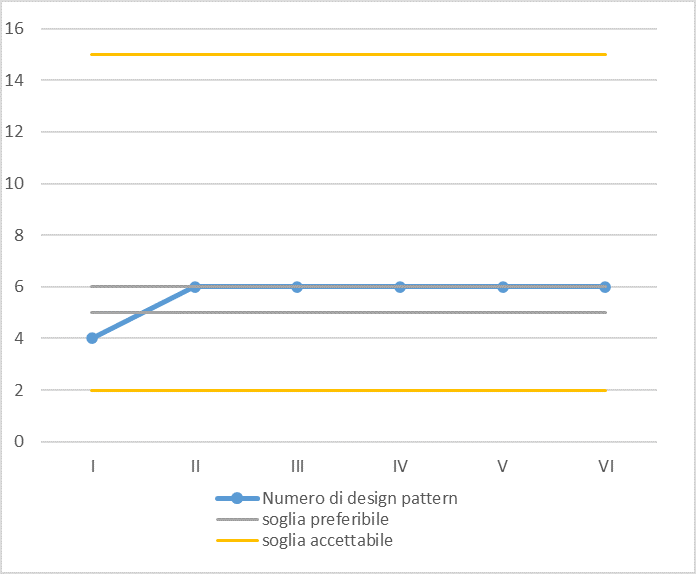
\includegraphics[width=\linewidth]{./img/grafici/RQ22.png}	
	\caption{M-PROC22 revisione di qualifica}	
\end{figure}
\begin{itemize}
	\item \textbf{Valore preferibile}: $5\le x \le 6$;
	\item \textbf{Valore accettabile}: $2 \le x \le 15$;
	\item \textbf{Considerazioni}: la metrica\glosp risulta soddisfatta al termine del periodo di qualifica.
\end{itemize}
\paragraph*{PRC-Q2 Processo di garanzia della qualità}
\subparagraph{M-PROC04 Percentuale di metriche soddisfatte} \mbox{}
\begin{longtable}[H!] {						
		>{}p{50mm}  		
		>{}p{8mm}
		>{}p{8mm}		
		>{}p{8mm}		
		>{}p{8mm}		
		>{}p{8mm}		
		>{}p{8mm}
		>{}p{8mm}
		>{}p{8mm}
		>{}p{8mm}
	}
	\rowcolor{gray!50}
	\textbf{} & \textbf{I} & \textbf{II} & \textbf{III} & \textbf{IV} & \textbf{V} & \textbf{VI}\TBstrut \\ [2mm]
	\textbf{Percentuale} & 88\% & 84\% & 92\% & 96\% & 92\% & 96\% \TBstrut \\ [2mm]
	\rowcolor{white}
	\caption{M-PROC04 revisione di qualifica}
\end{longtable}
\begin{figure}[H] 	
	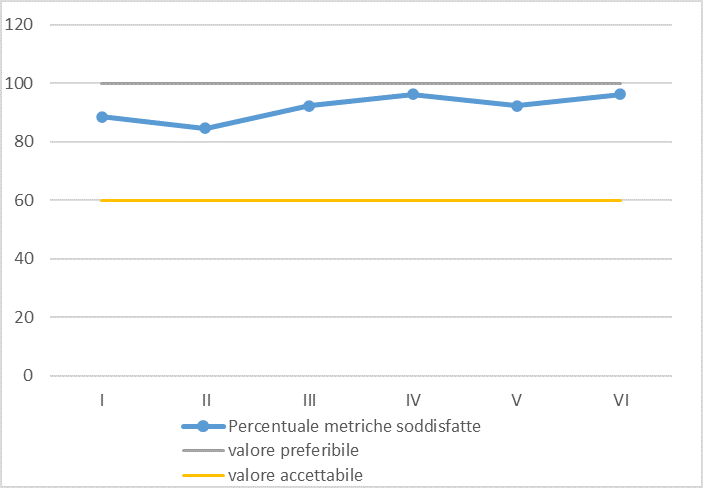
\includegraphics[width=\linewidth]{./img/grafici/RQ4.png}	
	\caption{M-PROC04 revisione di qualifica}	
\end{figure}
\begin{itemize}
	\item \textbf{Valore preferibile}: $=100\%$;
	\item \textbf{Valore accettabile}: $\ge60\%$;
	\item \textbf{Considerazioni}: la metrica\glosp risulta soddisfatta al termine del periodo di progettazione\glo.
\end{itemize}
\subparagraph{Considerazioni}
Il gruppo si ritiene soddisfatto rispetto al resoconto della verifica del periodo di qualifica visto il soddisfacimento della metrica M04. \\
Le metriche\glosp che non sono state soddisfatte al termine del VI periodo sono le seguenti:
\begin{itemize}
	\item \textbf{M-PROD16 Percentuale requisiti obbligatori soddisfatti}: il nostro prodotto\glo viene realizzato in modo incrementale, perciò in questo periodo questa metrica\glosp non è ancora soddisfatta. Nei prossimi periodi abbiamo pianificato di lavorare con gli incrementi necessari a soddisfare i requisiti obbligatori mancanti;
\end{itemize}  


\paragraph*{PRC-Q3 Processo di verifica}
\subparagraph{M-PROC05 Percentuale bug sistemati} \mbox{}
\begin{longtable}[H!] {						
		>{}p{50mm}  		
		>{}p{8mm}
		>{}p{8mm}		
		>{}p{8mm}		
		>{}p{8mm}		
		>{}p{8mm}		
		>{}p{8mm}
		>{}p{8mm}
		>{}p{8mm}
		>{}p{8mm}
	}
	\rowcolor{gray!50}
	\textbf{} & \textbf{I} & \textbf{II} & \textbf{III} & \textbf{IV} & \textbf{V} & \textbf{VI} \TBstrut \\ [2mm]
	\textbf{Percentuale} & 70\% & 80\% & 100\% & 100\% & 100\% & 100\% \TBstrut \\ [2mm]
	\rowcolor{white}
	\caption{M-PROC05 revisione di qualifica}
\end{longtable}
\begin{figure}[H] 	
	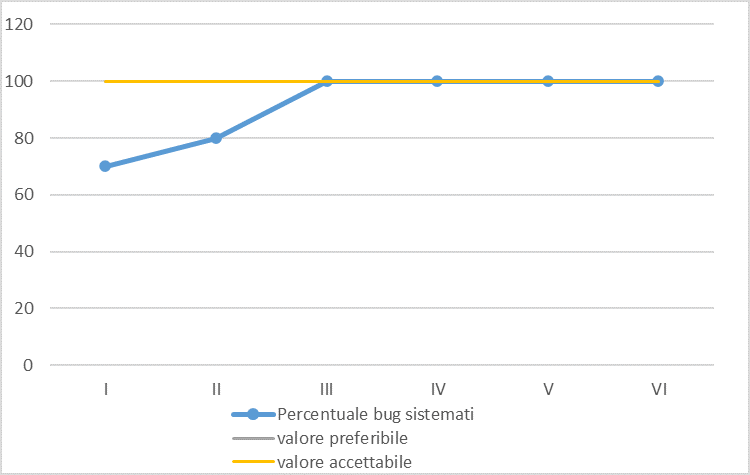
\includegraphics[width=\linewidth]{./img/grafici/RQ5.png}	
	\caption{M-PROC05 revisione di qualifica}	
\end{figure}
\begin{itemize}
	\item \textbf{Valore preferibile}: $=100\%$;
	\item \textbf{Valore accettabile}: $=100\%$;
	\item \textbf{Considerazioni}: la metrica\glosp risulta soddisfatta al termine del periodo di qualifica.
\end{itemize}

\subparagraph{M-PROC23 Code coverage} \mbox{}
\begin{longtable}[H!] {						
		>{}p{35mm}  		
		>{}p{12mm}
		>{}p{12mm}		
		>{}p{12mm}		
		>{}p{12mm}		
		>{}p{12mm}		
		>{}p{12mm}
		>{}p{12mm}
		>{}p{12mm}
		>{}p{12mm}
	}
	\rowcolor{gray!50}
	\textbf{} & \textbf{I} & \textbf{II} & \textbf{III} & \textbf{IV} & \textbf{V} & \textbf{VI} \TBstrut \\ [2mm]
	\textbf{Percentuale} & 80\% & 75\% & 88\% & 85\% & 87\% & 90\% \TBstrut \\ [2mm]
	\rowcolor{white}
	\caption{M-PROC23 revisione di qualifica}
\end{longtable}
\begin{figure}[H] 	
	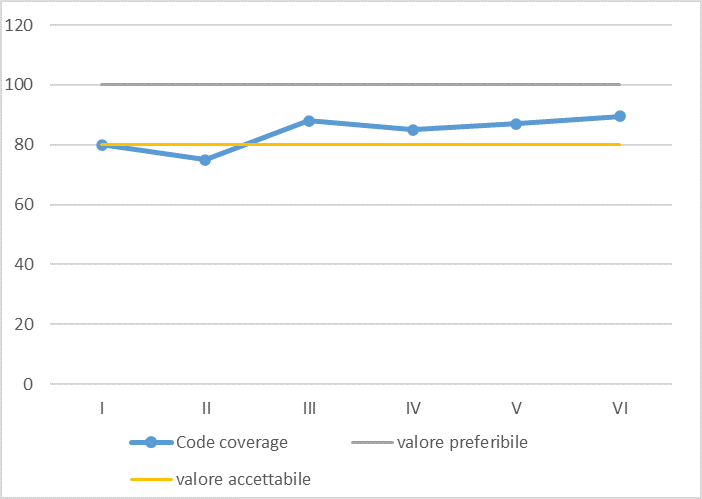
\includegraphics[width=\linewidth]{./img/grafici/RQ23.png}	
	\caption{M-PROC23 revisione di qualifica}	
\end{figure}
\begin{itemize}
	\item \textbf{Valore preferibile}: $=100\%$;
	\item \textbf{Valore accettabile}: $\ge 80\%$;
	\item \textbf{Considerazioni}: la metrica\glosp risulta soddisfatta al termine del periodo di qualifica.
\end{itemize}

\subparagraph{M-PROC24 Branch coverage} \mbox{}
\begin{longtable}[H!] {						
		>{}p{35mm}  		
		>{}p{12mm}
		>{}p{12mm}		
		>{}p{12mm}		
		>{}p{12mm}		
		>{}p{12mm}		
		>{}p{12mm}
		>{}p{12mm}
		>{}p{12mm}
		>{}p{12mm}
	}
	\rowcolor{gray!50}
	\textbf{} & \textbf{I} & \textbf{II} & \textbf{III} & \textbf{IV} & \textbf{V} & \textbf{VI} \TBstrut \\ [2mm]
	\textbf{Percentuale} & 79\% & 75\% & 80\% & 84\% & 86\% & 89\% \TBstrut \\ [2mm]
	\rowcolor{white}
	\caption{M-PROC24 revisione di qualifica}
\end{longtable}
\begin{figure}[H] 	
	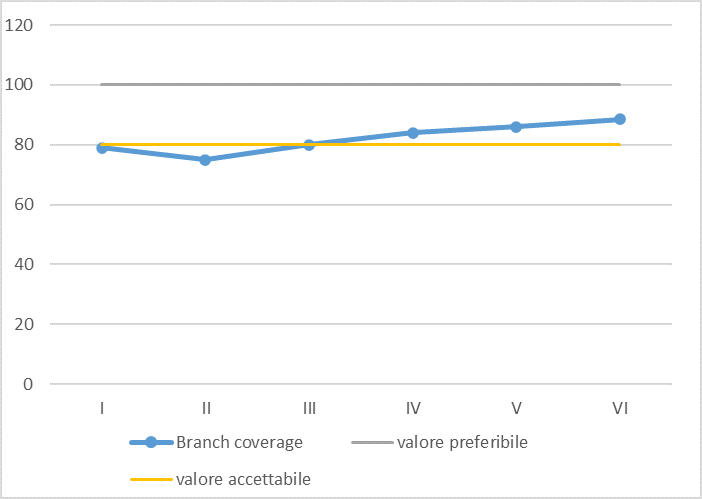
\includegraphics[width=\linewidth]{./img/grafici/RQ24.png}	
	\caption{M-PROC24 revisione di qualifica}	
\end{figure}
\begin{itemize}
	\item \textbf{Valore preferibile}: $=100\%$;
	\item \textbf{Valore accettabile}: $\ge 80\%$;
	\item \textbf{Considerazioni}: la metrica\glosp risulta soddisfatta al termine del periodo di qualifica.
\end{itemize}

\subparagraph{M-PROC25 Copertura test eseguiti} \mbox{}
\begin{longtable}[H!] {						
		>{}p{35mm}  		
		>{}p{12mm}
		>{}p{12mm}		
		>{}p{12mm}		
		>{}p{12mm}		
		>{}p{12mm}		
		>{}p{12mm}
		>{}p{12mm}
		>{}p{12mm}
		>{}p{12mm}
	}
	\rowcolor{gray!50}
	\textbf{} & \textbf{I} & \textbf{II} & \textbf{III} & \textbf{IV} & \textbf{V} & \textbf{VI} \TBstrut \\ [2mm]
	\textbf{Percentuale} & 100\% & 100\% & 100\% & 100\% & 100\% & 100\% \TBstrut \\ [2mm]
	\rowcolor{white}
	\caption{M-PROC25 revisione di qualifica}
\end{longtable}
\begin{figure}[H] 	
	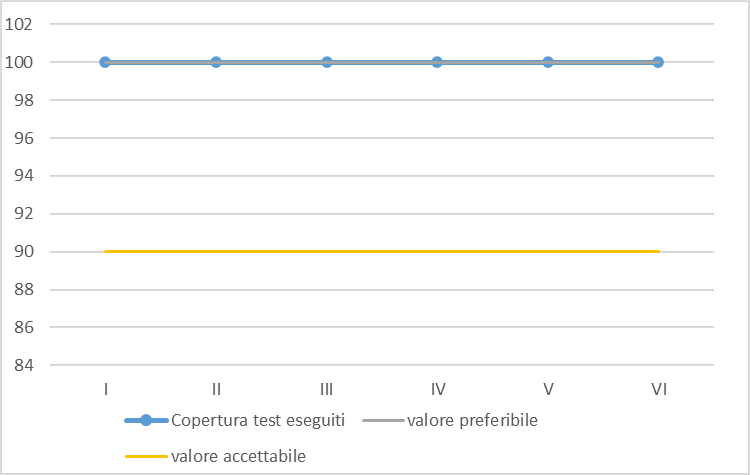
\includegraphics[width=\linewidth]{./img/grafici/RQ25.png}	
	\caption{M-PROC25 revisione di qualifica}	
\end{figure}
\begin{itemize}
	\item \textbf{Valore preferibile}: $100\%$
	\item \textbf{Valore accettabile}: $\ge 90\%$
	\item \textbf{Considerazioni}: la metrica\glosp risulta soddisfatta al termine del periodo di qualifica.
\end{itemize}

\paragraph*{PRC-Q4 Processo di gestione dei cambiamenti}
\subparagraph{M-PROC06 Tempo medio risoluzione errori} \mbox{}
\begin{longtable}[H!] {						
		>{}p{35mm}  		
		>{}p{12mm}
		>{}p{12mm}		
		>{}p{12mm}		
		>{}p{12mm}		
		>{}p{12mm}		
		>{}p{12mm}
		>{}p{12mm}
		>{}p{12mm}
		>{}p{12mm}
	}
	\rowcolor{gray!50}
	\textbf{} & \textbf{I} & \textbf{II} & \textbf{III} & \textbf{IV} & \textbf{V} & \textbf{VI} \TBstrut \\ [2mm]
	\textbf{Tempo medio} & 20min & 25min & 16min & 40min & 50min & 52min \TBstrut \\ [2mm]
	\rowcolor{white}
	\caption{M-PROC06 revisione di qualifica}
\end{longtable}
\begin{figure}[H] 	
	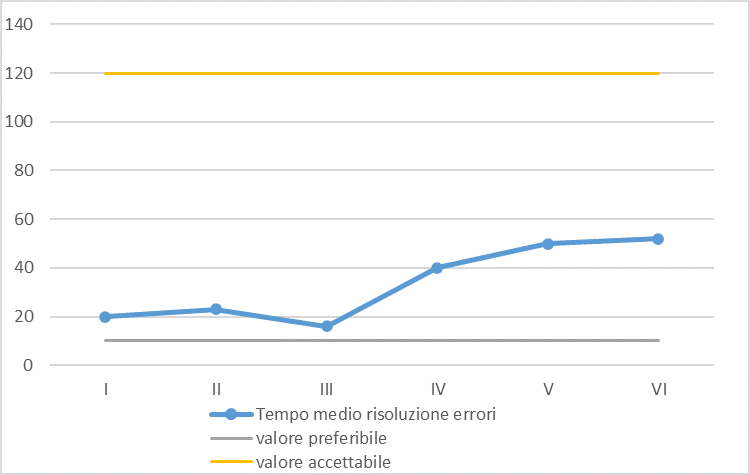
\includegraphics[width=\linewidth]{./img/grafici/RQ6.png}	
	\caption{M-PROC06 revisione di qualifica}	
\end{figure}
\begin{itemize}
	\item \textbf{Valore preferibile}: $\le10minuti$;
	\item \textbf{Valore accettabile}: $\le120minuti$;
	\item \textbf{Considerazioni}: la metrica\glosp risulta soddisfatta al termine del periodo di qualifica.
\end{itemize}

\paragraph*{PRC-Q5 Processo di gestione organizzativa}
\subparagraph{M-PROC07 Planned Value} \mbox{}
\begin{longtable}[H!] {						
		>{}p{35mm}  		
		>{}p{12mm}
		>{}p{12mm}		
		>{}p{12mm}		
		>{}p{12mm}		
		>{}p{12mm}		
		>{}p{12mm}
		>{}p{12mm}
		>{}p{12mm}
		>{}p{12mm}
	}
	\rowcolor{gray!50}
	\textbf{} & \textbf{I} & \textbf{II} & \textbf{III} & \textbf{IV} & \textbf{V} & \textbf{VI} \TBstrut \\ [2mm]
	\textbf{PV} & 2290\euro & 3830\euro & 4640\euro & 5185\euro & 6635\euro & 7160\euro \TBstrut \\ [2mm]
	\rowcolor{white}
	\caption{M-PROC07 revisione di qualifica}
\end{longtable}
\begin{figure}[H] 	
	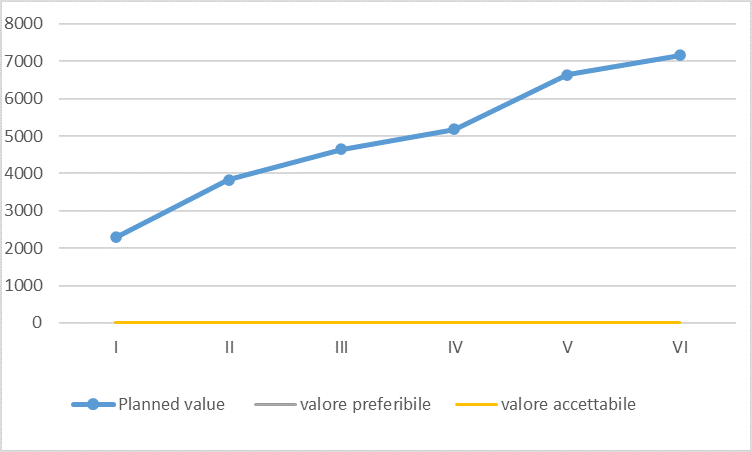
\includegraphics[width=\linewidth]{./img/grafici/RQ7.png}	
	\caption{M-PROC07 revisione di qualifica}	
\end{figure}
\begin{itemize}
	\item \textbf{Valore preferibile}: $\ge0$;
	\item \textbf{Valore accettabile}: $\ge0$;
	\item \textbf{Considerazioni}: la metrica\glosp risulta soddisfatta al termine del periodo di qualifica.
\end{itemize}

\subparagraph{M-PROC08 Earned Value} \mbox{}
\begin{longtable}[H!] {						
		>{}p{35mm}  		
		>{}p{12mm}
		>{}p{12mm}		
		>{}p{12mm}		
		>{}p{12mm}		
		>{}p{12mm}		
		>{}p{12mm}
		>{}p{12mm}
		>{}p{12mm}
		>{}p{12mm}
	}
	\rowcolor{gray!50}
	\textbf{} & \textbf{I} & \textbf{II} & \textbf{III} & \textbf{IV} & \textbf{V} & \textbf{VI} \TBstrut \\ [2mm]
	\textbf{EV} & 2290\euro & 3830\euro & 4640\euro & 5185\euro & 6635\euro & 7160\euro \TBstrut \\ [2mm]
	\rowcolor{white}
	\caption{M-PROC08 revisione di qualifica}
\end{longtable}
\begin{figure}[H] 	
	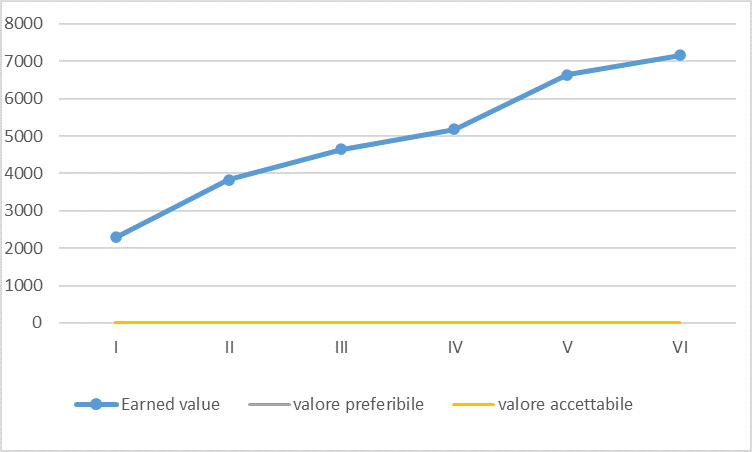
\includegraphics[width=\linewidth]{./img/grafici/RQ8.png}	
	\caption{M-PROC08 revisione di qualifica}	
\end{figure}
\begin{itemize}
	\item \textbf{Valore preferibile}: $\ge0$;
	\item \textbf{Valore accettabile}: $\ge0$;
	\item \textbf{Considerazioni}: la metrica\glosp risulta soddisfatta al termine del periodo di qualifica.
\end{itemize}

\subparagraph{M-PROC09 Actual Cost} \mbox{}
\begin{longtable}[H!] {						
		>{}p{35mm}  		
		>{}p{12mm}
		>{}p{12mm}		
		>{}p{12mm}		
		>{}p{12mm}		
		>{}p{12mm}		
		>{}p{12mm}
		>{}p{12mm}
		>{}p{12mm}
		>{}p{12mm}
	}
	\rowcolor{gray!50}
	\textbf{} & \textbf{I} & \textbf{II} & \textbf{III} & \textbf{IV} & \textbf{V} & \textbf{VI} \TBstrut \\ [2mm]
	\textbf{AC} & 2282\euro & 3778\euro & 4588\euro & 5155\euro & 6678\euro & 7159\euro \TBstrut \\ [2mm]
	\rowcolor{white}
	\caption{M-PROC09 revisione di qualifica}
\end{longtable}
\begin{figure}[H] 	
	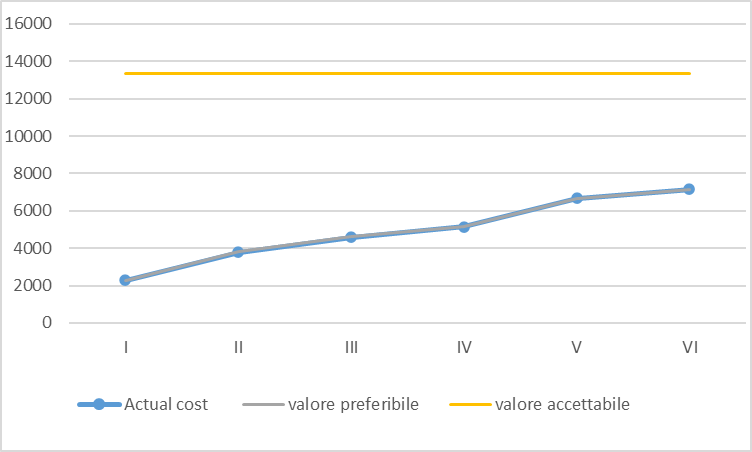
\includegraphics[width=\linewidth]{./img/grafici/RQ9.png}	
	\caption{M-PROC09 revisione di qualifica}	
\end{figure}
\begin{itemize}
	\item \textbf{Valore preferibile}: $0\le AC \le PV$;
	\item \textbf{Valore accettabile}: $0 \le AC \le budget \; totale$;
	\item \textbf{Considerazioni}: la metrica\glosp risulta soddisfatta al termine del periodo di qualifica.
\end{itemize}

\subparagraph{M-PROC10 Cost perform index} \mbox{}
\begin{longtable}[H!] {						
		>{}p{50mm}  		
		>{}p{8mm}
		>{}p{8mm}		
		>{}p{8mm}		
		>{}p{8mm}		
		>{}p{8mm}		
		>{}p{8mm}
		>{}p{8mm}
		>{}p{8mm}
		>{}p{8mm}
	}
	\rowcolor{gray!50}
	\textbf{} & \textbf{I} & \textbf{II} & \textbf{III} & \textbf{IV} & \textbf{V} & \textbf{VI} \TBstrut \\ [2mm]
	\textbf{CPI} & 1 & 1,01 & 1,01 & 1 & 0,99 & 1 \TBstrut \\ [2mm]
	\rowcolor{white}
	\caption{M-PROC10 revisione di qualifica}
\end{longtable}
\begin{figure}[H] 	
	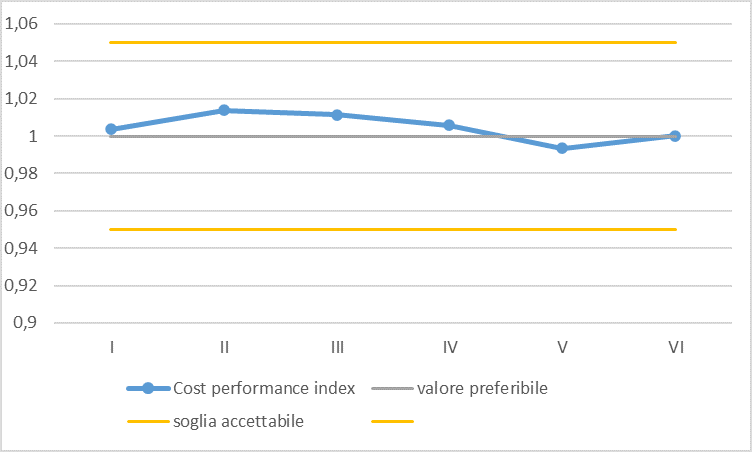
\includegraphics[width=\linewidth]{./img/grafici/RQ10.png}	
	\caption{M-PROC10 revisione di qualifica}	
\end{figure}
\begin{itemize}
	\item \textbf{Valore preferibile}: $=1$;
	\item \textbf{Valore accettabile}: $0.95 \le CPI \le 1.05$;
	\item \textbf{Considerazioni}: la metrica\glosp risulta soddisfatta al termine del periodo di qualifica.
\end{itemize}

\subparagraph{M-PROC11 Schedule perform index} \mbox{}
\begin{longtable}[H!] {						
		>{}p{50mm}  		
		>{}p{8mm}
		>{}p{8mm}		
		>{}p{8mm}		
		>{}p{8mm}		
		>{}p{8mm}		
		>{}p{8mm}
		>{}p{8mm}
		>{}p{8mm}
		>{}p{8mm}
	}
	\rowcolor{gray!50}
	\textbf{} & \textbf{I} & \textbf{II} & \textbf{III} & \textbf{IV} & \textbf{V} & \textbf{VI} \TBstrut \\ [2mm]
	\textbf{SPI} & 1 & 1 & 1 & 1 & 1 & 1 \TBstrut \\ [2mm]
	\rowcolor{white}
	\caption{M-PROC11 revisione di qualifica}
\end{longtable}
\begin{figure}[H] 	
	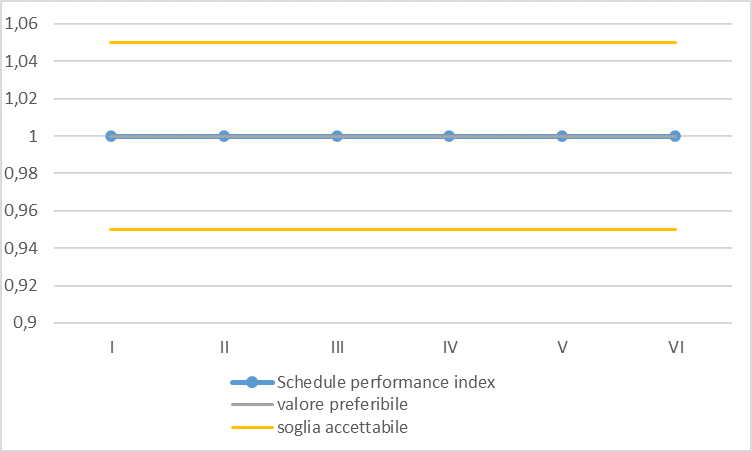
\includegraphics[width=\linewidth]{./img/grafici/RQ11.png}	
	\caption{M-PROC11 revisione di qualifica}	
\end{figure}
	\begin{itemize}
		\item \textbf{Valore preferibile}: $=1$;
		\item \textbf{Valore accettabile}: $0.95 \le SPI \le 1.05$;
		\item \textbf{Considerazioni}: la metrica\glosp risulta soddisfatta al termine del periodo di qualifica.
	\end{itemize}

\subparagraph{M-PROC12 Estimated cost at completion} \mbox{}
\begin{longtable}[H!] {						
		>{}p{35mm}  		
		>{}p{12mm}
		>{}p{12mm}		
		>{}p{12mm}		
		>{}p{12mm}		
		>{}p{12mm}		
		>{}p{12mm}
		>{}p{12mm}
		>{}p{12mm}
		>{}p{12mm}
	}
	\rowcolor{gray!50}
	\textbf{} & \textbf{I} & \textbf{II} & \textbf{III} & \textbf{IV} & \textbf{V} & \textbf{VI} \TBstrut \\ [2mm]
	\textbf{Costo} & 13333\euro & 13289\euro & 13289\euro & 13311\euro & 13384\euro & 13340\euro \TBstrut \\ [2mm]
	\rowcolor{white}
	\caption{M-PROC12 revisione di qualifica}
\end{longtable}
\begin{figure}[H] 	
	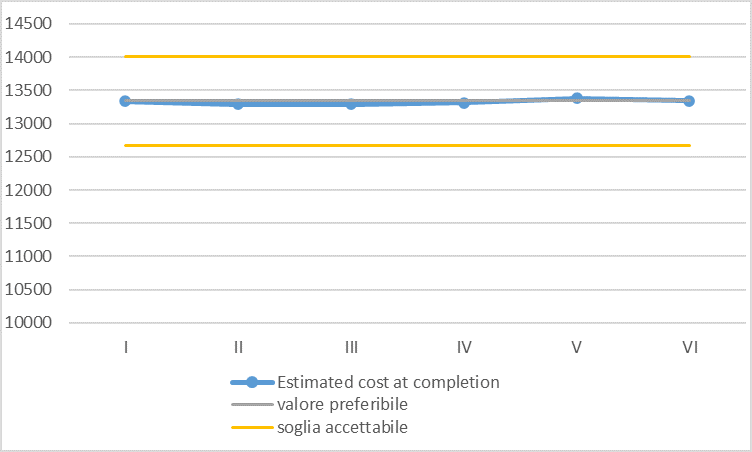
\includegraphics[width=\linewidth]{./img/grafici/RQ12.png}	
	\caption{M-PROC12 revisione di qualifica}	
\end{figure}
\begin{itemize}
	\item \textbf{Valore preferibile}: pari a quanto preventivato;
	\item \textbf{Valore accettabile}: $preventivo-5\% \le EAC \le preventivo+5\%$;
	\item \textbf{Considerazioni}: la metrica\glosp risulta soddisfatta al termine del periodo di qualifica.
\end{itemize}


\subparagraph{M-PROC13 Schedule at completion} \mbox{}
\begin{longtable}[H!] {						
		>{}p{15mm}  		
		>{}p{16mm}
		>{}p{16mm}		
		>{}p{16mm}		
		>{}p{16mm}		
		>{}p{16mm}		
		>{}p{16mm}
		>{}p{16mm}
		>{}p{16mm}
		>{}p{16mm}
	}
	\rowcolor{gray!50}
	\textbf{} & \textbf{I} & \textbf{II} & \textbf{III} & \textbf{IV} & \textbf{V} & \textbf{VI} \TBstrut \\ [2mm]
	\textbf{Ore} & 714 ore & 714 ore & 714 ore & 714 ore & 714 ore & 714 ore \TBstrut \\ [2mm]
	\rowcolor{white}
	\caption{M-PROC13 revisione di qualifica}
\end{longtable}
\begin{figure}[H] 	
	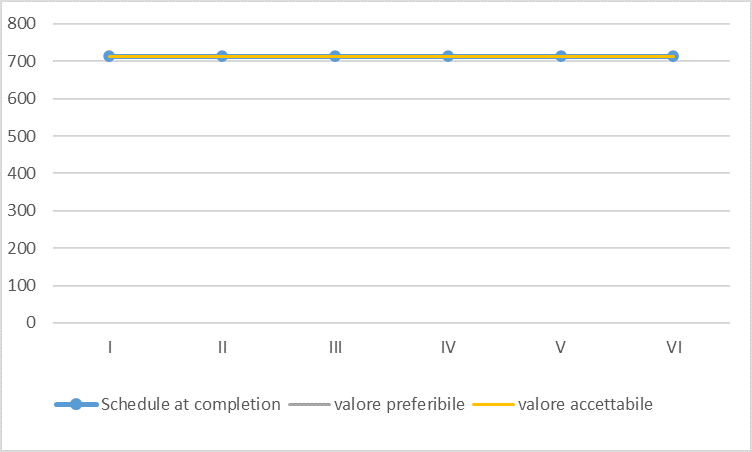
\includegraphics[width=\linewidth]{./img/grafici/RQ13.png}	
	\caption{M-PROC13 revisione di qualifica}	
\end{figure}
\begin{itemize}
	\item \textbf{Valore preferibile}: pari a quanto preventivato;
	\item \textbf{Valore accettabile}: pari a quanto preventivato;
	\item \textbf{Considerazioni}: la metrica\glosp risulta soddisfatta al termine del periodo di qualifica.
\end{itemize}

\subparagraph{M-PROC14 Rischi non preventivati} \mbox{}
\begin{longtable}[H!] {						
		>{}p{50mm}  		
		>{}p{8mm}
		>{}p{8mm}		
		>{}p{8mm}		
		>{}p{8mm}		
		>{}p{8mm}		
		>{}p{8mm}
		>{}p{8mm}
		>{}p{8mm}
		>{}p{8mm}
	}
	\rowcolor{gray!50}
	\textbf{} & \textbf{I} & \textbf{II} & \textbf{III} & \textbf{IV} & \textbf{V} & \textbf{VI} \TBstrut \\ [2mm]
	\textbf{Numero di rischi} & 0 & 0 & 0 & 0 & 0 & 0 \TBstrut \\ [2mm]
	\rowcolor{white}
	\caption{M-PROC14 revisione di qualifica}
\end{longtable}
\begin{figure}[H] 	
	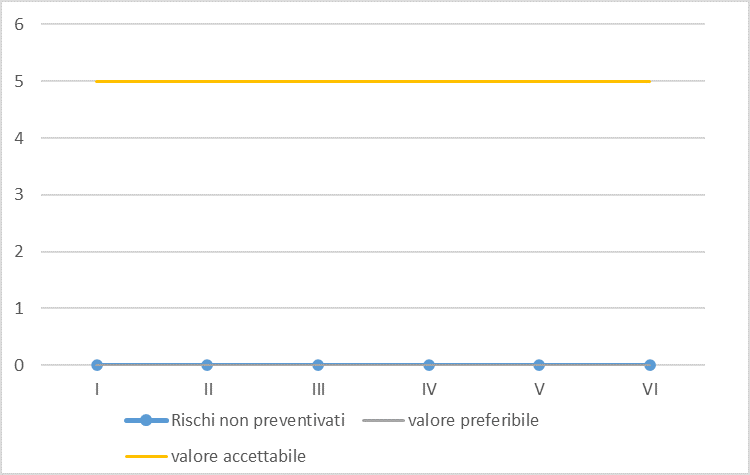
\includegraphics[width=\linewidth]{./img/grafici/RQ14.png}	
	\caption{M-PROC14 revisione di qualifica}	
\end{figure}
\begin{itemize}
	\item \textbf{Valore preferibile}: $=0$;
	\item \textbf{Valore accettabile}: $\le 5$;
	\item \textbf{Considerazioni}: la metrica\glosp risulta soddisfatta al termine del periodo di qualifica.
\end{itemize}

\paragraph{Qualità di prodotto}

\paragraph*{PRD-Q1 Documenti}
\subparagraph{M-PROD15 Indice di Gulpease}\mbox{}
\begin{longtable} {						
		>{}p{50mm}  		
		>{}p{8mm}		
		>{}p{8mm}		
		>{}p{8mm}		
		>{}p{8mm}		
		>{}p{8mm}		
		>{}p{8mm}
		>{}p{8mm}
		>{}p{8mm}
		>{}p{8mm}				
	}			
	\rowcolor{gray!50}
	\textbf{Documento} & \textbf{I} & \textbf{II} & \textbf{III} & \textbf{IV} & \textbf{V} & \textbf{VI} \TBstrut \\ [2mm]
	\textbf{Analisi dei Requisiti} & 100 & 100 & 100 & 100 & 100 & 100 \TBstrut \\ [2mm]
	\textbf{Norme di Progetto} & 84 & 82 & 79 & 86 & 83 & 81 \TBstrut \\ [2mm]
	\textbf{Piano di Progetto} & 98 & 97 & 94 & 96 & 93 & 100 \TBstrut \\ [2mm]
	\textbf{Piano di Qualifica} & 92 & 91 & 89 & 87 & 93 & 95 \TBstrut \\ [2mm]
	\textbf{Glossario} & 85 & 85 & 85 & 85 & 85 & 85 \TBstrut \\ [2mm]
	\textbf{Verbali interni (media)} & 86 & 87 & 90 & 88 & 90 & 90 \TBstrut \\ [2mm]
	\textbf{Verbali esterni (media)} & 84 & 84 & 84 & 84 & 88 & 88 \TBstrut \\ [2mm]
	\textbf{Manuale sviluppatore} & - & 85 & 87 & 75 & 84 & 81 \TBstrut \\ [2mm]
	\textbf{Manuale utente} & - & - & - & 84 & 86 & 88 \TBstrut \\ [2mm]
	\rowcolor{white}
	\caption{M-PROD15 revisione di qualifica}
\end{longtable}
\begin{figure}[H] 	
	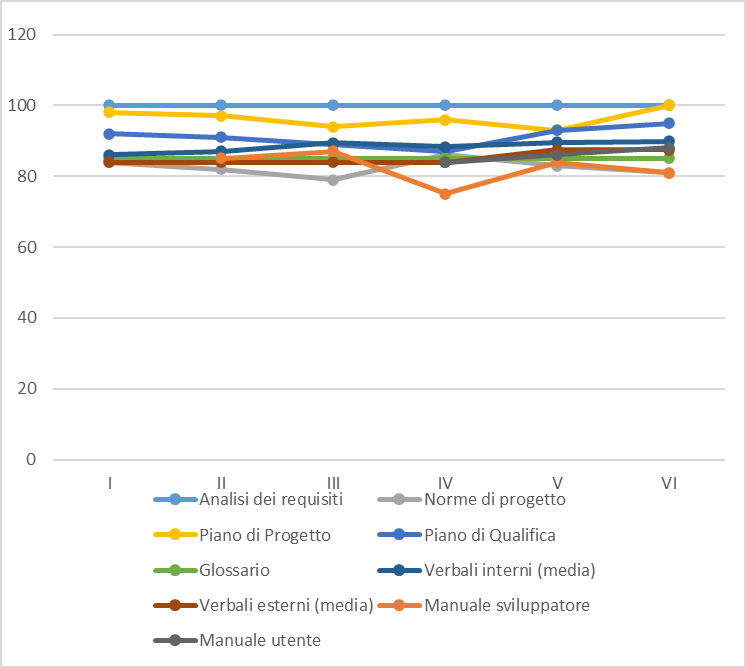
\includegraphics[width=\linewidth]{./img/grafici/RQ15a.png}	
	\caption{M-PROD15 revisione di qualifica}	
\end{figure}
\pagebreak
\begin{longtable} {						
		>{}p{70mm}  		
		>{}p{8mm}		
		>{}p{8mm}		
		>{}p{8mm}		
		>{}p{8mm}		
		>{}p{8mm}		
		>{}p{8mm}
		>{}p{8mm}
		>{}p{8mm}
		>{}p{8mm}				
	}			
	\rowcolor{gray!50}
	\textbf{} & \textbf{I} & \textbf{II} & \textbf{III} & \textbf{IV} & \textbf{V} & \textbf{VI} \TBstrut \\ [2mm]
	\textbf{Media dell'indice di Gulpease} & 90 & 89 & 89 & 87 & 89 & 90 \TBstrut \\ [2mm]
	\rowcolor{white}
	\caption{M-PROD15 revisione di qualifica}
\end{longtable}
\begin{figure}[H] 	
	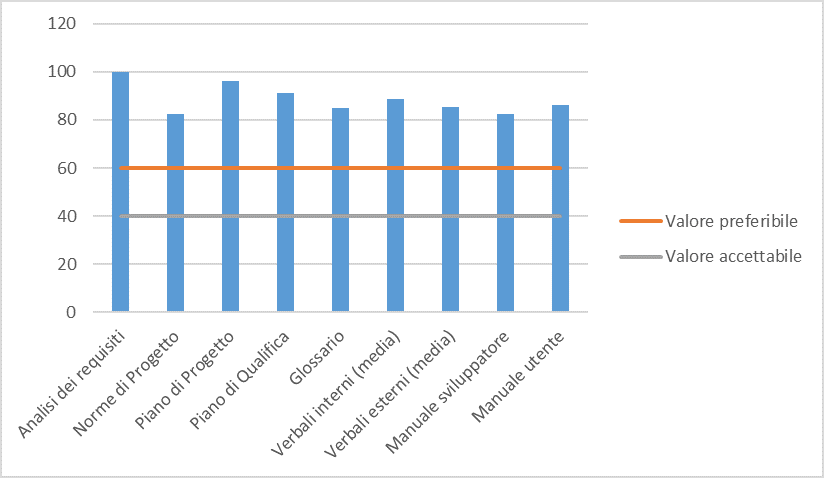
\includegraphics[width=\linewidth]{./img/grafici/RQ15b.png}	
	\caption{M-PROD15 revisione di qualifica}	
\end{figure}
\begin{itemize}
	\item \textbf{Valore preferibile}: $\ge60$;
	\item \textbf{Valore accettabile}: $\ge40$;
	\item \textbf{Considerazioni}: la metrica\glosp risulta soddisfatta al termine del periodo di qualifica.
\end{itemize}

\subparagraph{M-PROD19 Correttezza ortografica} \mbox{}
\begin{longtable}[H!] {						
		>{}p{50mm}  		
		>{}p{8mm}
		>{}p{8mm}		
		>{}p{8mm}		
		>{}p{8mm}		
		>{}p{8mm}		
		>{}p{8mm}
		>{}p{8mm}
		>{}p{8mm}
		>{}p{8mm}
	}
	\rowcolor{gray!50}
	\textbf{} & \textbf{I} & \textbf{II} & \textbf{III} & \textbf{IV} & \textbf{V} & \textbf{VI} \TBstrut \\ [2mm]
	\textbf{Numero errori} & 0 & 1 & 0 & 0 & 0 & 0 \TBstrut \\ [2mm]
	\rowcolor{white}
	\caption{M-PROD19 revisione di qualifica}
\end{longtable}
\begin{figure}[H] 	
	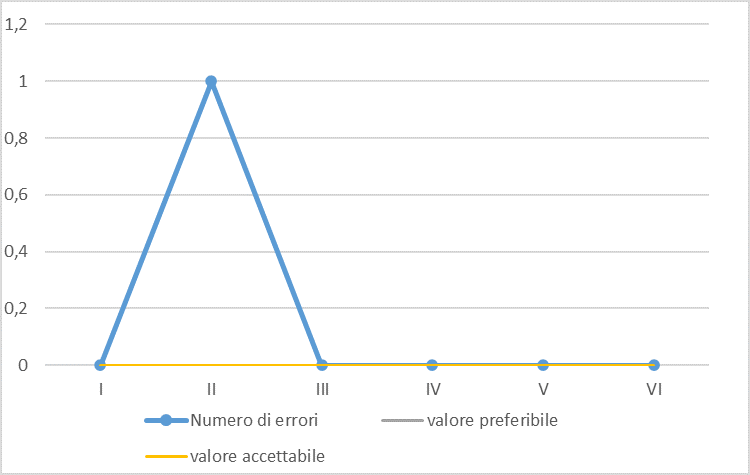
\includegraphics[width=\linewidth]{./img/grafici/RQ19.png}	
	\caption{M-PROD19 revisione di qualifica}	
\end{figure}
\begin{itemize}
	\item \textbf{Valore preferibile}: 0;
	\item \textbf{Valore accettabile}: 0;
	\item \textbf{Considerazioni}: la metrica\glosp risulta soddisfatta al termine del periodo di qualifica.
\end{itemize}


\paragraph*{PRD-Q2 Appropriatezza funzionale}
\subparagraph{M-PROD16 Percentuale requisiti obbligatori soddisfatti} \mbox{}
\begin{longtable}[H!] {						
		>{}p{50mm}  		
		>{}p{8mm}
		>{}p{8mm}		
		>{}p{8mm}		
		>{}p{8mm}		
		>{}p{8mm}		
		>{}p{8mm}
		>{}p{8mm}
		>{}p{8mm}
		>{}p{8mm}
	}
	\rowcolor{gray!50}
	\textbf{} & \textbf{I} & \textbf{II} & \textbf{III} & \textbf{IV} & \textbf{V} & \textbf{VI} \TBstrut \\ [2mm]
	\textbf{Percentuale} & 55\% & 58\% & 61\% & 68\% & 77\% & 87\% \TBstrut \\ [2mm]
	\rowcolor{white}
	\caption{M-PROD16 revisione di qualifica}
\end{longtable}
\begin{figure}[H] 	
	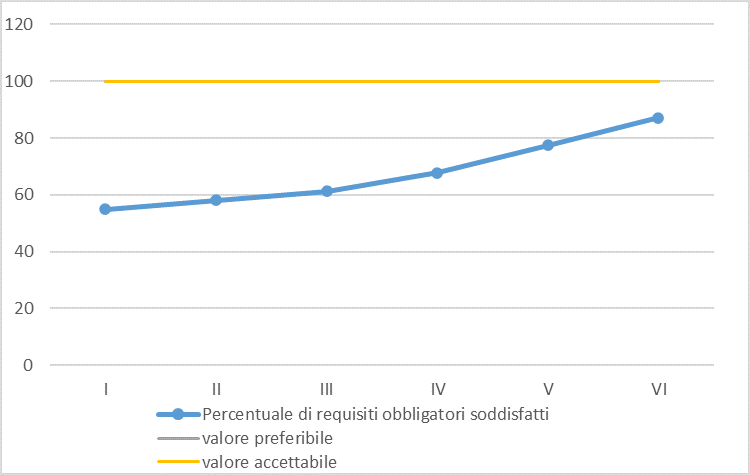
\includegraphics[width=\linewidth]{./img/grafici/RQ16.png}	
	\caption{M-PROD16 revisione di qualifica}	
\end{figure}
\begin{itemize}
	\item \textbf{Valore preferibile}: $=100\%$;
	\item \textbf{Valore accettabile}: $=100\%$;
	\item \textbf{Considerazioni}: la metrica\glosp risulta non soddisfatta al termine del periodo di qualifica.
\end{itemize}

\subparagraph{M-PROD17 Percentuale requisiti desiderabili soddisfatti} \mbox{}
\begin{longtable}[H!] {						
		>{}p{50mm}  		
		>{}p{8mm}
		>{}p{8mm}		
		>{}p{8mm}		
		>{}p{8mm}		
		>{}p{8mm}		
		>{}p{8mm}
		>{}p{8mm}
		>{}p{8mm}
		>{}p{8mm}
	}
	\rowcolor{gray!50}
	\textbf{} & \textbf{I} & \textbf{II} & \textbf{III} & \textbf{IV} & \textbf{V} & \textbf{VI} \TBstrut \\ [2mm]
	\textbf{Percentuale} & 9\% & 9\% & 9\% & 9\% & 9\% & 9\% \TBstrut \\ [2mm]
	\rowcolor{white}
	\caption{M-PROD17 revisione di qualifica}
\end{longtable}
\begin{figure}[H] 	
	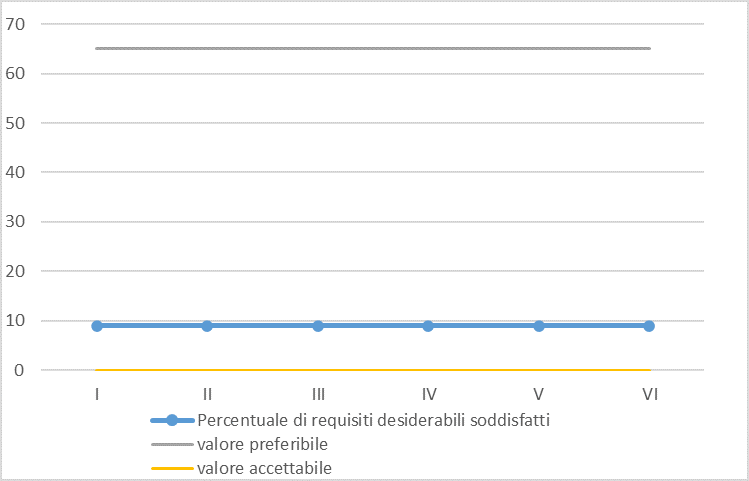
\includegraphics[width=\linewidth]{./img/grafici/RQ17.png}	
	\caption{M-PROD17 revisione di qualifica}	
\end{figure}
\begin{itemize}
	\item \textbf{Valore preferibile}: $\ge 65\%$;
	\item \textbf{Valore accettabile}: $\ge 0\%$;
	\item \textbf{Considerazioni}: la metrica\glosp risulta soddisfatta al termine del periodo di qualifica.
\end{itemize}

\subparagraph{M-PROD18 Percentuale requisiti opzionali soddisfatti} \mbox{}
\begin{longtable}[H!] {						
		>{}p{50mm}  		
		>{}p{8mm}
		>{}p{8mm}		
		>{}p{8mm}		
		>{}p{8mm}		
		>{}p{8mm}		
		>{}p{8mm}
		>{}p{8mm}
		>{}p{8mm}
		>{}p{8mm}
	}
	\rowcolor{gray!50}
	\textbf{} & \textbf{I} & \textbf{II} & \textbf{III} & \textbf{IV} & \textbf{V} & \textbf{VI} \TBstrut \\ [2mm]
	\textbf{Percentuale} & 0\% & 0\% & 0\% & 0\% & 0\% & 0\% \TBstrut \\ [2mm]
	\rowcolor{white}
	\caption{M-PROD18 revisione di qualifica}
\end{longtable}
\begin{figure}[H] 	
	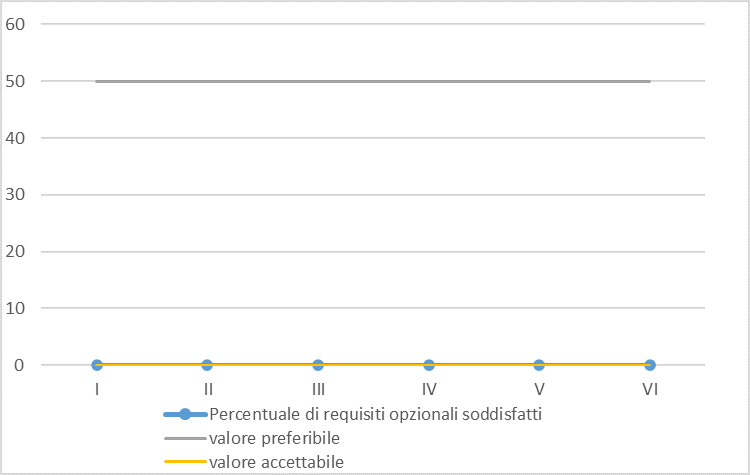
\includegraphics[width=\linewidth]{./img/grafici/RQ18.png}	
	\caption{M-PROD18 revisione di qualifica}	
\end{figure}
\begin{itemize}
	\item \textbf{Valore preferibile}: $\ge 50\%$;
	\item \textbf{Valore accettabile}: $\ge 0\%$;
	\item \textbf{Considerazioni}: la metrica\glosp risulta soddisfatta al termine del periodo di qualifica.
\end{itemize}

\subparagraph{M-PROD26 Percentuale test passati} \mbox{}
\begin{longtable}[H!] {						
		>{}p{50mm}  		
		>{}p{8mm}
		>{}p{8mm}		
		>{}p{8mm}		
		>{}p{8mm}		
		>{}p{8mm}		
		>{}p{8mm}
		>{}p{8mm}
		>{}p{8mm}
		>{}p{8mm}
	}
	\rowcolor{gray!50}
	\textbf{} & \textbf{I} & \textbf{II} & \textbf{III} & \textbf{IV} & \textbf{V} & \textbf{VI} \TBstrut \\ [2mm]
	\textbf{Percentuale} & 83\% & 100\% & 79\% & 98\% & 100\% & 100\% \TBstrut \\ [2mm]
	\rowcolor{white}
	\caption{M-PROD26 revisione di qualifica}
\end{longtable}
\begin{figure}[H] 	
	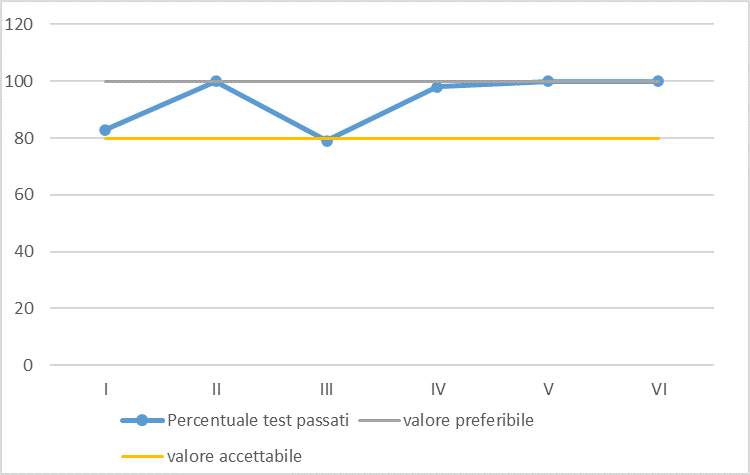
\includegraphics[width=\linewidth]{./img/grafici/RQ26.png}	
	\caption{M-PROD26 revisione di qualifica}	
\end{figure}
\begin{itemize}
	\item \textbf{Valore preferibile}: $= 100\%$;
	\item \textbf{Valore accettabile}: $\ge 80\%$;
	\item \textbf{Considerazioni}: la metrica\glosp risulta soddisfatta al termine del periodo di qualifica.
\end{itemize}


\subsection{Revisione di accettazione (RA)}
\subsubsection{Riassunto delle attività di verifica}
In questo periodo abbiamo attuato le verifiche sui documenti, sulla codifica, sulla pianificazione, sulla progettazione e sui test per verificare che lo svolgimento del progetto\glosp procedesse senza impedimenti.  
\paragraph{Analisi statica dei documenti}
L'analisi statica\glosp dei documenti ha portato alla produzione di una lista degli errori comuni ridotti rispetto alla revisione precedente.
\subsubsection{Esiti delle verifiche} 
\paragraph{Qualità di processo}
\paragraph*{PRC-Q1 Processo di sviluppo}
\subparagraph{M-PROC01 Scostamento dei requisiti individuati} \mbox{}
\begin{longtable}[H!] {						
		>{}p{50mm}  		
		>{}p{8mm}
		>{}p{8mm}		
		>{}p{8mm}		
	}
	\rowcolor{gray!50}
	\textbf{} & \textbf{I} & \textbf{II} & \textbf{III}  \TBstrut \\ [2mm]
	\textbf{Scostamenti} & 0 & 0 & 0 \TBstrut \\ [2mm]
	\rowcolor{white}
	\caption{M-PROC01 revisione di validazione e collaudo}
\end{longtable}
\begin{figure}[H] 	
	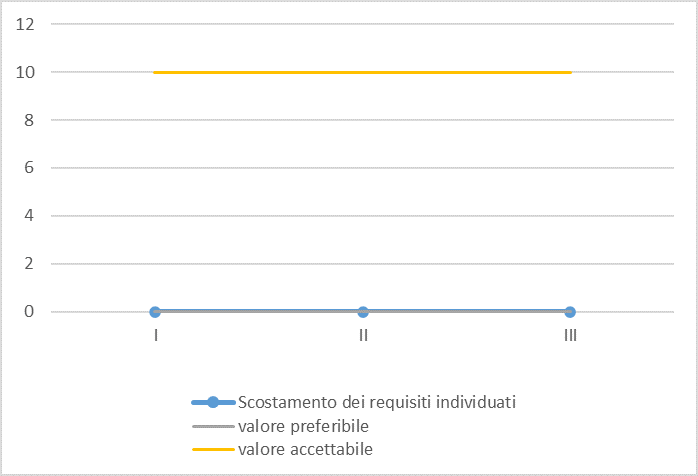
\includegraphics[width=\linewidth]{./img/grafici/RA1.png}	
	\caption{M-PROC01 revisione di validazione e collaudo}	
\end{figure}
\begin{itemize}
	\item \textbf{Valore preferibile}: 0;
	\item \textbf{Valore accettabile}: 10;
	\item \textbf{Considerazioni}: la metrica\glosp risulta soddisfatta al termine del periodo di qualifica.
\end{itemize}

\subparagraph{M-PROC02 Numero di parametri per metodo} \mbox{}
\begin{longtable}[H!] {						
		>{}p{50mm}  		
		>{}p{8mm}
		>{}p{8mm}		
		>{}p{8mm}		
	}
	\rowcolor{gray!50}
	\textbf{} & \textbf{I} & \textbf{II} & \textbf{III} \TBstrut \\ [2mm]
	\textbf{Numero} & 5 & 5 & 5 \TBstrut \\ [2mm]
	\rowcolor{white}
	\caption{M-PROC02 revisione di validazione e collaudo}
\end{longtable}
\begin{figure}[H] 	
	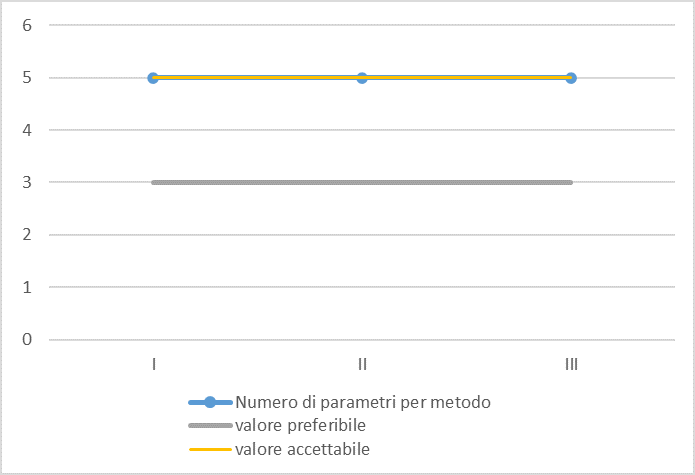
\includegraphics[width=\linewidth]{./img/grafici/RA2.png}	
	\caption{M-PROC02 revisione di validazione e collaudo}	
\end{figure}
\begin{itemize}
	\item \textbf{Valore preferibile}: $\le 3$;
	\item \textbf{Valore accettabile}: $\le 5$;
	\item \textbf{Considerazioni}: la metrica\glosp risulta soddisfatta al termine del periodo di qualifica.
\end{itemize}

\subparagraph{M-PROC03 Numero di metodi per classe} \mbox{}
\begin{longtable}[H!] {						
		>{}p{50mm}  		
		>{}p{8mm}
		>{}p{8mm}		
		>{}p{8mm}		
	}
	\rowcolor{gray!50}
	\textbf{} & \textbf{I} & \textbf{II} & \textbf{III} \TBstrut \\ [2mm]
	\textbf{Numero} & 15 & 15 & 15 \TBstrut \\ [2mm]
	\rowcolor{white}
	\caption{M-PROC03 revisione di validazione e collaudo}
\end{longtable}
\begin{figure}[H] 	
	\includegraphics[width=\linewidth]{./img/grafici/RA3.png}	
	\caption{M-PROC03 revisione di validazione e collaudo}	
\end{figure}
\begin{itemize}
	\item \textbf{Valore preferibile}: $\le 8$;
	\item \textbf{Valore accettabile}: $\le 15$;
	\item \textbf{Considerazioni}: la metrica\glosp risulta soddisfatta al termine del periodo di qualifica.
\end{itemize}

\subparagraph{M-PROC20 Livello di annidamento} \mbox{}
\begin{longtable}[H!] {						
		>{}p{50mm}  		
		>{}p{8mm}
		>{}p{8mm}		
		>{}p{8mm}		
	}
	\rowcolor{gray!50}
	\textbf{} & \textbf{I} & \textbf{II} & \textbf{III} \TBstrut \\ [2mm]
	\textbf{Livello} & 2 & 2 & 2 \TBstrut \\ [2mm]
	\rowcolor{white}
	\caption{M-PROC20 revisione di validazione e collaudo}
\end{longtable}
\begin{figure}[H] 	
	\includegraphics[width=\linewidth]{./img/grafici/RA20.png}	
	\caption{M-PROC20 revisione di validazione e collaudo}	
\end{figure}
\begin{itemize}
	\item \textbf{Valore preferibile}: $1\le x \le 3$;
	\item \textbf{Valore accettabile}: $1 \le x \le 7$;
	\item \textbf{Considerazioni}: la metrica\glosp risulta soddisfatta al termine del periodo di qualifica.
\end{itemize}
\subparagraph{M-PROC21 Profondità gerarchia} \mbox{}
\begin{longtable}[H!] {						
		>{}p{50mm}  		
		>{}p{8mm}
		>{}p{8mm}		
		>{}p{8mm}		
	}
	\rowcolor{gray!50}
	\textbf{} & \textbf{I} & \textbf{II} & \textbf{III} \TBstrut \\ [2mm]
	\textbf{Profondità} & 2 & 2 & 2 \TBstrut \\ [2mm]
	\rowcolor{white}
	\caption{M-PROC21 revisione di validazione e collaudo}
\end{longtable}
\begin{figure}[H] 	
	\includegraphics[width=\linewidth]{./img/grafici/RA21.png}	
	\caption{M-PROC21 revisione di validazione e collaudo}	
\end{figure}
\begin{itemize}
	\item \textbf{Valore preferibile}: $\le 4$;
	\item \textbf{Valore accettabile}: $\le 7$;
	\item \textbf{Considerazioni}: la metrica\glosp risulta soddisfatta al termine del periodo di qualifica.
\end{itemize}

\subparagraph{M-PROC22 Numero di design pattern} \mbox{}
\begin{longtable}[H!] {						
		>{}p{50mm}  		
		>{}p{8mm}
		>{}p{8mm}		
		>{}p{8mm}		
	}
	\rowcolor{gray!50}
	\textbf{} & \textbf{I} & \textbf{II} & \textbf{III} \TBstrut \\ [2mm]
	\textbf{Numero} & 6 & 6 & 6 \TBstrut \\ [2mm]
	\rowcolor{white}
	\caption{M-PROC22 revisione di validazione e collaudo}
\end{longtable}
\begin{figure}[H] 	
	\includegraphics[width=\linewidth]{./img/grafici/RA22.png}	
	\caption{M-PROC22 revisione di validazione e collaudo}	
\end{figure}
\begin{itemize}
	\item \textbf{Valore preferibile}: $5\le x \le 6$;
	\item \textbf{Valore accettabile}: $2 \le x \le 15$;
	\item \textbf{Considerazioni}: la metrica\glosp risulta soddisfatta al termine del periodo di qualifica.
\end{itemize}
\paragraph*{PRC-Q2 Processo di garanzia della qualità}
\subparagraph{M-PROC04 Percentuale di metriche soddisfatte} \mbox{}
\begin{longtable}[H!] {						
		>{}p{50mm}  		
		>{}p{8mm}
		>{}p{8mm}		
		>{}p{8mm}		
	}
	\rowcolor{gray!50}
	\textbf{} & \textbf{I} & \textbf{II} & \textbf{III}\TBstrut \\ [2mm]
	\textbf{Percentuale} & 100\% & 100\% & 100\% \TBstrut \\ [2mm]
	\rowcolor{white}
	\caption{M-PROC04 revisione di validazione e collaudo}
\end{longtable}
\begin{figure}[H] 	
	\includegraphics[width=\linewidth]{./img/grafici/RA4.png}	
	\caption{M-PROC04 revisione di validazione e collaudo}	
\end{figure}
\begin{itemize}
	\item \textbf{Valore preferibile}: $=100\%$;
	\item \textbf{Valore accettabile}: $\ge60\%$;
	\item \textbf{Considerazioni}: la metrica\glosp risulta soddisfatta al termine del periodo di progettazione\glo.
\end{itemize}
\subparagraph{Considerazioni}
Il gruppo si ritiene pienamente soddisfatto rispetto al resoconto della verifica del periodo di qualifica visto il raggiungimento del valore preferibile della metrica M04. 


\paragraph*{PRC-Q3 Processo di verifica}
\subparagraph{M-PROC05 Percentuale bug sistemati} \mbox{}
\begin{longtable}[H!] {						
		>{}p{50mm}  		
		>{}p{8mm}
		>{}p{8mm}		
		>{}p{8mm}		
	}
	\rowcolor{gray!50}
	\textbf{} & \textbf{I} & \textbf{II} & \textbf{III} \TBstrut \\ [2mm]
	\textbf{Percentuale} & 100\% & 100\% & 100\% \TBstrut \\ [2mm]
	\rowcolor{white}
	\caption{M-PROC05 revisione di validazione e collaudo}
\end{longtable}
\begin{figure}[H] 	
	\includegraphics[width=\linewidth]{./img/grafici/RA5.png}	
	\caption{M-PROC05 revisione di validazione e collaudo}	
\end{figure}
\begin{itemize}
	\item \textbf{Valore preferibile}: $=100\%$;
	\item \textbf{Valore accettabile}: $=100\%$;
	\item \textbf{Considerazioni}: la metrica\glosp risulta soddisfatta al termine del periodo di qualifica.
\end{itemize}

\subparagraph{M-PROC23 Code coverage} \mbox{}
\begin{longtable}[H!] {						
		>{}p{35mm}  		
		>{}p{12mm}
		>{}p{12mm}		
		>{}p{12mm}		
	}
	\rowcolor{gray!50}
	\textbf{} & \textbf{I} & \textbf{II} & \textbf{III} \TBstrut \\ [2mm]
	\textbf{Percentuale} & 94\% & 95\% & 97\% \TBstrut \\ [2mm]
	\rowcolor{white}
	\caption{M-PROC23 revisione di validazione e collaudo}
\end{longtable}
\begin{figure}[H] 	
	\includegraphics[width=\linewidth]{./img/grafici/RA23.png}	
	\caption{M-PROC23 revisione di validazione e collaudo}	
\end{figure}
\begin{itemize}
	\item \textbf{Valore preferibile}: $=100\%$;
	\item \textbf{Valore accettabile}: $\ge 80\%$;
	\item \textbf{Considerazioni}: la metrica\glosp risulta soddisfatta al termine del periodo di qualifica.
\end{itemize}

\subparagraph{M-PROC24 Branch coverage} \mbox{}
\begin{longtable}[H!] {						
		>{}p{35mm}  		
		>{}p{12mm}
		>{}p{12mm}		
		>{}p{12mm}		
	}
	\rowcolor{gray!50}
	\textbf{} & \textbf{I} & \textbf{II} & \textbf{III} \TBstrut \\ [2mm]
	\textbf{Percentuale} & 92\% & 94\% & 95\% \TBstrut \\ [2mm]
	\rowcolor{white}
	\caption{M-PROC24 revisione di validazione e collaudo}
\end{longtable}
\begin{figure}[H] 	
	\includegraphics[width=\linewidth]{./img/grafici/RA24.png}	
	\caption{M-PROC24 revisione di validazione e collaudo}	
\end{figure}
\begin{itemize}
	\item \textbf{Valore preferibile}: $=100\%$;
	\item \textbf{Valore accettabile}: $\ge 80\%$;
	\item \textbf{Considerazioni}: la metrica\glosp risulta soddisfatta al termine del periodo di qualifica.
\end{itemize}

\subparagraph{M-PROC25 Copertura test eseguiti} \mbox{}
\begin{longtable}[H!] {						
		>{}p{35mm}  		
		>{}p{12mm}
		>{}p{12mm}		
		>{}p{12mm}		
	}
	\rowcolor{gray!50}
	\textbf{} & \textbf{I} & \textbf{II} & \textbf{III} \TBstrut \\ [2mm]
	\textbf{Percentuale} & 100\% & 100\% & 100\% \TBstrut \\ [2mm]
	\rowcolor{white}
	\caption{M-PROC25 revisione di validazione e collaudo}
\end{longtable}
\begin{figure}[H] 	
	\includegraphics[width=\linewidth]{./img/grafici/RA25.png}	
	\caption{M-PROC25 revisione di validazione e collaudo}	
\end{figure}
\begin{itemize}
	\item \textbf{Valore preferibile}: $100\%$
	\item \textbf{Valore accettabile}: $\ge 90\%$
	\item \textbf{Considerazioni}: la metrica\glosp risulta soddisfatta al termine del periodo di qualifica.
\end{itemize}

\paragraph*{PRC-Q4 Processo di gestione dei cambiamenti}
\subparagraph{M-PROC06 Tempo medio risoluzione errori} \mbox{}
\begin{longtable}[H!] {						
		>{}p{35mm}  		
		>{}p{12mm}
		>{}p{12mm}		
		>{}p{12mm}		
		>{}p{12mm}		
		>{}p{12mm}		
		>{}p{12mm}
		>{}p{12mm}
		>{}p{12mm}
		>{}p{12mm}
	}
	\rowcolor{gray!50}
	\textbf{} & \textbf{I} & \textbf{II} & \textbf{III} \TBstrut \\ [2mm]
	\textbf{Tempo medio} & 35min & 38min & 25min  \TBstrut \\ [2mm]
	\rowcolor{white}
	\caption{M-PROC06 revisione di validazione e collaudo}
\end{longtable}
\begin{figure}[H] 	
	\includegraphics[width=\linewidth]{./img/grafici/RQ6.png}	
	\caption{M-PROC06 revisione di validazione e collaudo}	
\end{figure}
\begin{itemize}
	\item \textbf{Valore preferibile}: $\le10minuti$;
	\item \textbf{Valore accettabile}: $\le120minuti$;
	\item \textbf{Considerazioni}: la metrica\glosp risulta soddisfatta al termine del periodo di qualifica.
\end{itemize}

\paragraph*{PRC-Q5 Processo di gestione organizzativa}
\subparagraph{M-PROC07 Planned Value} \mbox{}
\begin{longtable}[H!] {						
		>{}p{35mm}  		
		>{}p{12mm}
		>{}p{12mm}		
		>{}p{12mm}		
	}
	\rowcolor{gray!50}
	\textbf{} & \textbf{I} & \textbf{II} & \textbf{III} \TBstrut \\ [2mm]
	\textbf{PV} & 1033\euro & 1735\euro & 2345\euro  \TBstrut \\ [2mm]
	\rowcolor{white}
	\caption{M-PROC07 revisione di validazione e collaudo}
\end{longtable}
\begin{figure}[H] 	
	\includegraphics[width=\linewidth]{./img/grafici/RA7.png}	
	\caption{M-PROC07 revisione di validazione e collaudo}	
\end{figure}
\begin{itemize}
	\item \textbf{Valore preferibile}: $\ge0$;
	\item \textbf{Valore accettabile}: $\ge0$;
	\item \textbf{Considerazioni}: la metrica\glosp risulta soddisfatta al termine del periodo di qualifica.
\end{itemize}

\subparagraph{M-PROC08 Earned Value} \mbox{}
\begin{longtable}[H!] {						
		>{}p{35mm}  		
		>{}p{12mm}
		>{}p{12mm}		
		>{}p{12mm}		
	}
	\rowcolor{gray!50}
	\textbf{} & \textbf{I} & \textbf{II} & \textbf{III} \TBstrut \\ [2mm]
	\textbf{EV} & 1033\euro & 1735\euro & 2345\euro  \TBstrut \\ [2mm]
	\rowcolor{white}
	\caption{M-PROC08 revisione di validazione e collaudo}
\end{longtable}
\begin{figure}[H] 	
	\includegraphics[width=\linewidth]{./img/grafici/RA8.png}	
	\caption{M-PROC08 revisione di validazione e collaudo}	
\end{figure}
\begin{itemize}
	\item \textbf{Valore preferibile}: $\ge0$;
	\item \textbf{Valore accettabile}: $\ge0$;
	\item \textbf{Considerazioni}: la metrica\glosp risulta soddisfatta al termine del periodo di qualifica.
\end{itemize}

\subparagraph{M-PROC09 Actual Cost} \mbox{}
\begin{longtable}[H!] {						
		>{}p{35mm}  		
		>{}p{12mm}
		>{}p{12mm}		
		>{}p{12mm}		
	}
	\rowcolor{gray!50}
	\textbf{} & \textbf{I} & \textbf{II} & \textbf{III}  \TBstrut \\ [2mm]
	\textbf{AC} & 1011\euro & 1743\euro & 2333\euro  \TBstrut \\ [2mm]
	\rowcolor{white}
	\caption{M-PROC09 revisione di validazione e collaudo}
\end{longtable}
\begin{figure}[H] 	
	\includegraphics[width=\linewidth]{./img/grafici/RA9.png}	
	\caption{M-PROC09 revisione di validazione e collaudo}	
\end{figure}
\begin{itemize}
	\item \textbf{Valore preferibile}: $0\le AC \le PV$;
	\item \textbf{Valore accettabile}: $0 \le AC \le budget \; totale$;
	\item \textbf{Considerazioni}: la metrica\glosp risulta soddisfatta al termine del periodo di qualifica.
\end{itemize}

\subparagraph{M-PROC10 Cost perform index} \mbox{}
\begin{longtable}[H!] {						
		>{}p{50mm}  		
		>{}p{8mm}
		>{}p{8mm}		
		>{}p{8mm}		
	}
	\rowcolor{gray!50}
	\textbf{} & \textbf{I} & \textbf{II} & \textbf{III}  \TBstrut \\ [2mm]
	\textbf{CPI} & 1,02 & 0,99 & 1 \TBstrut \\ [2mm]
	\rowcolor{white}
	\caption{M-PROC10 revisione di validazione e collaudo}
\end{longtable}
\begin{figure}[H] 	
	\includegraphics[width=\linewidth]{./img/grafici/RA10.png}	
	\caption{M-PROC10 revisione di validazione e collaudo}	
\end{figure}
\begin{itemize}
	\item \textbf{Valore preferibile}: $=1$;
	\item \textbf{Valore accettabile}: $0.95 \le CPI \le 1.05$;
	\item \textbf{Considerazioni}: la metrica\glosp risulta soddisfatta al termine del periodo di qualifica.
\end{itemize}

\subparagraph{M-PROC11 Schedule perform index} \mbox{}
\begin{longtable}[H!] {						
		>{}p{50mm}  		
		>{}p{8mm}
		>{}p{8mm}		
		>{}p{8mm}		
	}
	\rowcolor{gray!50}
	\textbf{} & \textbf{I} & \textbf{II} & \textbf{III} \TBstrut \\ [2mm]
	\textbf{SPI} & 1 & 1 & 1 \TBstrut \\ [2mm]
	\rowcolor{white}
	\caption{M-PROC11 revisione di validazione e collaudo}
\end{longtable}
\begin{figure}[H] 	
	\includegraphics[width=\linewidth]{./img/grafici/RA11.png}	
	\caption{M-PROC11 revisione di validazione e collaudo}	
\end{figure}
\begin{itemize}
	\item \textbf{Valore preferibile}: $=1$;
	\item \textbf{Valore accettabile}: $0.95 \le SPI \le 1.05$;
	\item \textbf{Considerazioni}: la metrica\glosp risulta soddisfatta al termine del periodo di qualifica.
\end{itemize}

\subparagraph{M-PROC12 Estimated cost at completion} \mbox{}
\begin{longtable}[H!] {						
		>{}p{35mm}  		
		>{}p{12mm}
		>{}p{12mm}		
		>{}p{12mm}		
	}
	\rowcolor{gray!50}
	\textbf{} & \textbf{I} & \textbf{II} & \textbf{III}  \TBstrut \\ [2mm]
	\textbf{Costo} & 13319\euro & 13349\euro & 13329\euro \TBstrut \\ [2mm]
	\rowcolor{white}
	\caption{M-PROC12 revisione di validazione e collaudo}
\end{longtable}
\begin{figure}[H] 	
	\includegraphics[width=\linewidth]{./img/grafici/RA12.png}	
	\caption{M-PROC12 revisione di validazione e collaudo}	
\end{figure}
\begin{itemize}
	\item \textbf{Valore preferibile}: pari a quanto preventivato;
	\item \textbf{Valore accettabile}: $preventivo-5\% \le EAC \le preventivo+5\%$;
	\item \textbf{Considerazioni}: la metrica\glosp risulta soddisfatta al termine del periodo di qualifica.
\end{itemize}


\subparagraph{M-PROC13 Schedule at completion} \mbox{}
\begin{longtable}[H!] {						
		>{}p{15mm}  		
		>{}p{16mm}
		>{}p{16mm}		
		>{}p{16mm}		
	}
	\rowcolor{gray!50}
	\textbf{} & \textbf{I} & \textbf{II} & \textbf{III}  \TBstrut \\ [2mm]
	\textbf{Ore} & 714 ore & 714 ore & 714 ore  \TBstrut \\ [2mm]
	\rowcolor{white}
	\caption{M-PROC13 revisione di validazione e collaudo}
\end{longtable}
\begin{figure}[H] 	
	\includegraphics[width=\linewidth]{./img/grafici/RA13.png}	
	\caption{M-PROC13 revisione di validazione e collaudo}	
\end{figure}
\begin{itemize}
	\item \textbf{Valore preferibile}: pari a quanto preventivato;
	\item \textbf{Valore accettabile}: pari a quanto preventivato;
	\item \textbf{Considerazioni}: la metrica\glosp risulta soddisfatta al termine del periodo di qualifica.
\end{itemize}

\subparagraph{M-PROC14 Rischi non preventivati} \mbox{}
\begin{longtable}[H!] {						
		>{}p{50mm}  		
		>{}p{8mm}
		>{}p{8mm}		
		>{}p{8mm}		
	}
	\rowcolor{gray!50}
	\textbf{} & \textbf{I} & \textbf{II} & \textbf{III}  \TBstrut \\ [2mm]
	\textbf{Numero di rischi} & 0 & 0 & 0  \TBstrut \\ [2mm]
	\rowcolor{white}
	\caption{M-PROC14 revisione di validazione e collaudo}
\end{longtable}
\begin{figure}[H] 	
	\includegraphics[width=\linewidth]{./img/grafici/RA14.png}	
	\caption{M-PROC14 revisione di validazione e collaudo}	
\end{figure}
\begin{itemize}
	\item \textbf{Valore preferibile}: $=0$;
	\item \textbf{Valore accettabile}: $\le 5$;
	\item \textbf{Considerazioni}: la metrica\glosp risulta soddisfatta al termine del periodo di qualifica.
\end{itemize}

\subparagraph{M-PROD27 Percentuale test alta priorità implementati} \mbox{}
\begin{longtable}[H!] {						
		>{}p{50mm}  		
		>{}p{8mm}
		>{}p{8mm}		
		>{}p{8mm}		
	}
	\rowcolor{gray!50}
	\textbf{} & \textbf{I} & \textbf{II} & \textbf{III}  \TBstrut \\ [2mm]
	\textbf{Percentuale} & 93\% & 100\% & 100\%  \TBstrut \\ [2mm]
	\rowcolor{white}
	\caption{M-PROC27 revisione di validazione e collaudo}
\end{longtable}
\begin{figure}[H] 	
	\includegraphics[width=\linewidth]{./img/grafici/RA27.png}	
	\caption{M-PROC27 revisione di validazione e collaudo}	
\end{figure}
\begin{itemize}
	\item \textbf{Valore preferibile}: $= 100\%$;
	\item \textbf{Valore accettabile}: $= 100\%$;
	\item \textbf{Considerazioni}: la metrica\glosp risulta soddisfatta al termine del periodo di qualifica.
\end{itemize}

\subparagraph{M-PROC27 Percentuale test alta priorità implementati} \mbox{}
\begin{longtable}[H!] {						
		>{}p{50mm}  		
		>{}p{8mm}
		>{}p{8mm}		
		>{}p{8mm}		
	}
	\rowcolor{gray!50}
	\textbf{} & \textbf{I} & \textbf{II} & \textbf{III}  \TBstrut \\ [2mm]
	\textbf{Percentuale} & 92\% & 92\% & 100\%  \TBstrut \\ [2mm]
	\rowcolor{white}
	\caption{M-PROC28 revisione di validazione e collaudo}
\end{longtable}
\begin{figure}[H] 	
	\includegraphics[width=\linewidth]{./img/grafici/RA28.png}	
	\caption{M-PROC28 revisione di validazione e collaudo}	
\end{figure}
\begin{itemize}
	\item \textbf{Valore preferibile}: $\ge 85\%$;
	\item \textbf{Valore accettabile}: $= 100\%$;
	\item \textbf{Considerazioni}: la metrica\glosp risulta soddisfatta al termine del periodo di qualifica.
\end{itemize}

\paragraph{Qualità di prodotto}

\paragraph*{PRD-Q1 Documenti}
\subparagraph{M-PROD15 Indice di Gulpease}\mbox{}
\begin{longtable} {						
		>{}p{50mm}  		
		>{}p{8mm}		
		>{}p{8mm}		
		>{}p{8mm}		
		>{}p{8mm}		
		>{}p{8mm}		
		>{}p{8mm}
		>{}p{8mm}
		>{}p{8mm}
		>{}p{8mm}				
	}			
	\rowcolor{gray!50}
	\textbf{Documento} & \textbf{I} & \textbf{II} & \textbf{III} & \textbf{IV} & \textbf{V} & \textbf{VI} \TBstrut \\ [2mm]
	\textbf{Analisi dei Requisiti} & 100 & 100 & 100 & 100 & 100 & 100 \TBstrut \\ [2mm]
	\textbf{Norme di Progetto} & 84 & 82 & 79 & 86 & 83 & 81 \TBstrut \\ [2mm]
	\textbf{Piano di Progetto} & 98 & 97 & 94 & 96 & 93 & 100 \TBstrut \\ [2mm]
	\textbf{Piano di Qualifica} & 92 & 91 & 89 & 87 & 93 & 95 \TBstrut \\ [2mm]
	\textbf{Glossario} & 85 & 85 & 85 & 85 & 85 & 85 \TBstrut \\ [2mm]
	\textbf{Verbali interni (media)} & 86 & 87 & 90 & 88 & 90 & 90 \TBstrut \\ [2mm]
	\textbf{Verbali esterni (media)} & 84 & 84 & 84 & 84 & 88 & 88 \TBstrut \\ [2mm]
	\textbf{Manuale sviluppatore} & - & 85 & 87 & 75 & 84 & 81 \TBstrut \\ [2mm]
	\textbf{Manuale utente} & - & - & - & 84 & 86 & 88 \TBstrut \\ [2mm]
	\rowcolor{white}
	\caption{M-PROD15 revisione di qualifica}
\end{longtable}
\begin{figure}[H] 	
	\includegraphics[width=\linewidth]{./img/grafici/RQ15a.png}	
	\caption{M-PROD15 revisione di qualifica}	
\end{figure}
\pagebreak
\begin{longtable} {						
		>{}p{70mm}  		
		>{}p{8mm}		
		>{}p{8mm}		
		>{}p{8mm}		
		>{}p{8mm}		
		>{}p{8mm}		
		>{}p{8mm}
		>{}p{8mm}
		>{}p{8mm}
		>{}p{8mm}				
	}			
	\rowcolor{gray!50}
	\textbf{} & \textbf{I} & \textbf{II} & \textbf{III} & \textbf{IV} & \textbf{V} & \textbf{VI} \TBstrut \\ [2mm]
	\textbf{Media dell'indice di Gulpease} & 90 & 89 & 89 & 87 & 89 & 90 \TBstrut \\ [2mm]
	\rowcolor{white}
	\caption{M-PROD15 revisione di qualifica}
\end{longtable}
\begin{figure}[H] 	
	\includegraphics[width=\linewidth]{./img/grafici/RQ15b.png}	
	\caption{M-PROD15 revisione di qualifica}	
\end{figure}
\begin{itemize}
	\item \textbf{Valore preferibile}: $\ge60$;
	\item \textbf{Valore accettabile}: $\ge40$;
	\item \textbf{Considerazioni}: la metrica\glosp risulta soddisfatta al termine del periodo di qualifica.
\end{itemize}

\subparagraph{M-PROD19 Correttezza ortografica} \mbox{}
\begin{longtable}[H!] {						
		>{}p{50mm}  		
		>{}p{8mm}
		>{}p{8mm}		
		>{}p{8mm}		
	}
	\rowcolor{gray!50}
	\textbf{} & \textbf{I} & \textbf{II} & \textbf{III}  \TBstrut \\ [2mm]
	\textbf{Numero errori} & 0 & 0 & 0  \TBstrut \\ [2mm]
	\rowcolor{white}
	\caption{M-PROD19 revisione di validazione e collaudo}
\end{longtable}
\begin{figure}[H] 	
	\includegraphics[width=\linewidth]{./img/grafici/RA19.png}	
	\caption{M-PROD19 revisione di validazione e collaudo}	
\end{figure}
\begin{itemize}
	\item \textbf{Valore preferibile}: 0;
	\item \textbf{Valore accettabile}: 0;
	\item \textbf{Considerazioni}: la metrica\glosp risulta soddisfatta al termine del periodo di qualifica.
\end{itemize}


\paragraph*{PRD-Q2 Appropriatezza funzionale}
\subparagraph{M-PROD16 Percentuale requisiti obbligatori soddisfatti} \mbox{}
\begin{longtable}[H!] {						
		>{}p{50mm}  		
		>{}p{8mm}
		>{}p{8mm}		
		>{}p{8mm}		
	}
	\rowcolor{gray!50}
	\textbf{} & \textbf{I} & \textbf{II} & \textbf{III} \TBstrut \\ [2mm]
	\textbf{Percentuale} & 100\% & 100\% & 100\%  \TBstrut \\ [2mm]
	\rowcolor{white}
	\caption{M-PROD16 revisione di validazione e collaudo}
\end{longtable}
\begin{figure}[H] 	
	\includegraphics[width=\linewidth]{./img/grafici/RA16.png}	
	\caption{M-PROD16 revisione di validazione e collaudo}	
\end{figure}
\begin{itemize}
	\item \textbf{Valore preferibile}: $=100\%$;
	\item \textbf{Valore accettabile}: $=100\%$;
	\item \textbf{Considerazioni}: la metrica\glosp risulta soddisfatta al termine del periodo di qualifica.
\end{itemize}

\subparagraph{M-PROD17 Percentuale requisiti desiderabili soddisfatti} \mbox{}
\begin{longtable}[H!] {						
		>{}p{50mm}  		
		>{}p{8mm}
		>{}p{8mm}		
		>{}p{8mm}		
	}
	\rowcolor{gray!50}
	\textbf{} & \textbf{I} & \textbf{II} & \textbf{III} \TBstrut \\ [2mm]
	\textbf{Percentuale} & 9\% & 100\% & 100\%  \TBstrut \\ [2mm]
	\rowcolor{white}
	\caption{M-PROD17 revisione di validazione e collaudo}
\end{longtable}
\begin{figure}[H] 	
	\includegraphics[width=\linewidth]{./img/grafici/RA17.png}	
	\caption{M-PROD17 revisione di validazione e collaudo}	
\end{figure}
\begin{itemize}
	\item \textbf{Valore preferibile}: $\ge 65\%$;
	\item \textbf{Valore accettabile}: $\ge 0\%$;
	\item \textbf{Considerazioni}: la metrica\glosp risulta soddisfatta al termine del periodo di qualifica.
\end{itemize}

\subparagraph{M-PROD18 Percentuale requisiti opzionali soddisfatti} \mbox{}
\begin{longtable}[H!] {						
		>{}p{50mm}  		
		>{}p{8mm}
		>{}p{8mm}		
		>{}p{8mm}		
		>{}p{8mm}		
		>{}p{8mm}		
		>{}p{8mm}
		>{}p{8mm}
		>{}p{8mm}
		>{}p{8mm}
	}
	\rowcolor{gray!50}
	\textbf{} & \textbf{I} & \textbf{II} & \textbf{III}  \TBstrut \\ [2mm]
	\textbf{Percentuale} & 0\% & 0\% & 0\%  \TBstrut \\ [2mm]
	\rowcolor{white}
	\caption{M-PROD18 revisione di validazione e collaudo}
\end{longtable}
\begin{figure}[H] 	
	\includegraphics[width=\linewidth]{./img/grafici/RA18.png}	
	\caption{M-PROD18 revisione di validazione e collaudo}	
\end{figure}
\begin{itemize}
	\item \textbf{Valore preferibile}: $\ge 50\%$;
	\item \textbf{Valore accettabile}: $\ge 0\%$;
	\item \textbf{Considerazioni}: la metrica\glosp risulta soddisfatta al termine del periodo di qualifica.
\end{itemize}

\subparagraph{M-PROD26 Percentuale test passati} \mbox{}
\begin{longtable}[H!] {						
		>{}p{50mm}  		
		>{}p{8mm}
		>{}p{8mm}		
		>{}p{8mm}		
	}
	\rowcolor{gray!50}
	\textbf{} & \textbf{I} & \textbf{II} & \textbf{III}  \TBstrut \\ [2mm]
	\textbf{Percentuale} & 100\% & 100\% & 100\%  \TBstrut \\ [2mm]
	\rowcolor{white}
	\caption{M-PROD26 revisione di validazione e collaudo}
\end{longtable}
\begin{figure}[H] 	
	\includegraphics[width=\linewidth]{./img/grafici/RA26.png}	
	\caption{M-PROD26 revisione di validazione e collaudo}	
\end{figure}
\begin{itemize}
	\item \textbf{Valore preferibile}: $= 100\%$;
	\item \textbf{Valore accettabile}: $\ge 80\%$;
	\item \textbf{Considerazioni}: la metrica\glosp risulta soddisfatta al termine del periodo di qualifica.
\end{itemize}


\subsubsection{Revisioni generali}\mbox{}
\begin{longtable} {						
		>{}p{30mm}  		
		>{}p{15mm}		
		>{}p{15mm}		
		>{}p{15mm}		
		>{}p{15mm}						
	}			
	\rowcolor{gray!50}
	\textbf{Metrica} & \textbf{RR} & \textbf{RP} & \textbf{RQ} & \textbf{RA} \TBstrut \\ [2mm]
	\textbf{M-PROC01} & - & 29 & 0 & 0 \TBstrut \\ [2mm]
	\textbf{M-PROC02} & - & 4 & 5 & 5 \TBstrut \\ [2mm]
	\textbf{M-PROC03} & - & 21 & 15 & 15 \TBstrut \\ [2mm]
	\textbf{M-PROC04} & - & 78\% & 96\% & 100\% \TBstrut \\ [2mm]
	\textbf{M-PROC05} & - & 40\% & 100\% & 100\% \TBstrut \\ [2mm]
	\textbf{M-PROC06} & - & 104 min & 52 min & 25 min \TBstrut \\ [2mm]
	\textbf{M-PROC07} & - & 3836\euro & 7160\euro & 2345\euro \TBstrut \\ [2mm]
	\textbf{M-PROC08} & - & 3836\euro & 7160\euro & 2345\euro \TBstrut \\ [2mm]
	\textbf{M-PROC09} & - & 3836\euro & 7159\euro & 2333\euro \TBstrut \\ [2mm]
	\textbf{M-PROC10} & - & 1 & 1 & 1 \TBstrut \\ [2mm]
	\textbf{M-PROC11} & - & 1 & 1 & 1 \TBstrut \\ [2mm]
	\textbf{M-PROC12} & - & 13341\euro & 13340\euro & 13329\euro \TBstrut \\ [2mm]
	\textbf{M-PROC13} & - & 714 ore & 714 ore & 714 ore \TBstrut \\ [2mm]
	\textbf{M-PROC14} & - & 0 & 0 & 0 \TBstrut \\ [2mm]	
	\textbf{M-PROD15} & 82 & 93 & 90 & - \TBstrut \\ [2mm]
	\textbf{M-PROD16} & - & 53\% & 87\% & 100\% \TBstrut \\ [2mm]
	\textbf{M-PROD17} & - & 0 & 9\% & 100\% \TBstrut \\ [2mm]
	\textbf{M-PROD18} & - & 0\% & 0\% & 0\% \TBstrut \\ [2mm]
	\textbf{M-PROD19} & - & 0 & 0 & 0 \TBstrut \\ [2mm]
	\textbf{M-PROC20} & - & - & 2 & 2 \TBstrut \\ [2mm]
	\textbf{M-PROC21} & - & - & 2 & 2 \TBstrut \\ [2mm]
	\textbf{M-PROC22} & - & - & 6 & 6 \TBstrut \\ [2mm]
	\textbf{M-PROC23} & - & - & 90\% & 97\% \TBstrut \\ [2mm]
	\textbf{M-PROC24} & - & - & 89\% & 95 \TBstrut \\ [2mm]
	\textbf{M-PROC25} & - & - & 100 & 100\% \TBstrut \\ [2mm]
	\textbf{M-PROD26} & - & - & 100 & 100\% \TBstrut \\ [2mm]
	\textbf{M-PROC27} & - & - & - & 100\% \TBstrut \\ [2mm]
	\textbf{M-PROC28} & - & - & - & 100\% \TBstrut \\ [2mm]
	\rowcolor{white}
	\caption{Revisione generale}
\end{longtable}
